\documentclass[12pt, a4paper]{article}

\usepackage{fancyhdr}
\usepackage{float}
\usepackage[left=2cm, right=2cm, top=2cm, bottom=2cm]{geometry}
\usepackage{graphicx}
\usepackage[utf8]{inputenc}
\usepackage{amsmath}
\usepackage{amssymb}
\usepackage{amsthm}
\usepackage{enumerate}
\usepackage[most]{tcolorbox}
\usepackage{tikz}
\usepackage{caption}
\usepackage{hyperref}
\usepackage{diagbox}

\newcommand{\doctitle}{MATH 318 Notes}
\newcommand{\name}{Jimmy Yang}

\pagestyle{fancy}
\lhead{\textbf{\doctitle}}

\newcounter{exa}

\tcbset{
myexample/.style={
  enhanced,
  breakable,
  colback=yellow!10!white,
  colframe=red!50!black,
  fonttitle=\scshape,
  titlerule=0pt,
  title={\refstepcounter{exa}example~\theexa.},
  title style={fill=yellow!10!white},
  coltitle=red!50!black,
  drop shadow,
  highlight math style={reset,colback=LightBlue!50!white,colframe=Navy}
  frame hidden,
  }
}

\newtcolorbox{texample}{myexample}

\newtheorem*{theorem}{Theorem}

% disable indentation
\setlength\parindent{0pt}

\begin{document}

\begin{flushright}
\name
\end{flushright}

\begin{center}
\Large
\bfseries
\doctitle
\end{center}

% suppress the fancy header on the first page only
\thispagestyle{plain}

\begin{center}
Notes for MATH 318: Probability with Physical Applications. Contains additional stuff and examples from other places that are not covered during classes. If you have any questions or comments related to the notes, free to email me at \href{mailto:marethyu@student.ubc.ca}{marethyu@student.ubc.ca}. \\
Last modified: \today
\end{center}

\tableofcontents

\section{Counting}

\subsection{Permutations}

Permutations are combinations where order matters. How permutations are calculated depends on whether repetitions are allowed or not. The number of permutations made from choosing $k$ from $n$ items when repetitions are allowed is $n^k$.

\begin{texample}
Find the number of permutations of $ab$ when letters can be repeated. \\

The permutations are: $aa, ab, ba, bb$. There is a total of $2^2=4$ permutations.
\end{texample}

When repetitions are not allowed, the number of permutations is just $n!$. Here is one way to understand where this formula came from: for the first item, there are $n$ choices to place and since no repetitions are allowed, there are $n-1$ choices left for the second item and so on.

\begin{texample}
An Olympic final consists of two runners from each of four different countries. An ordered selection of three of the eight runners win the medals (gold, silver, and bronze). How many different possibilities are there if the medal winners are all from different countries? \\

We are looking for an ordered selection of winners. There are $8$ choices for the gold medal winner. After the winner is chosen, since we want winners from different countries, there are $6$ options left for the solver medal winner. This leaves with $4$ options for the bronze medal winner. The total number of possible selections is therefore $8\times6\times4=192$.
\end{texample}

\begin{texample}
Find the number of permutations of $abc$. \\

The permutations are: $abc, acb, bac, bca, cab, cba$. There are total of $3(2!)=3!=6$ permutations. Three unique letters times the number of permutations of remaining letters. If there are 4 letters, the answer would be $4(3!)=24$.
\end{texample}

\begin{figure}[H]
\centering
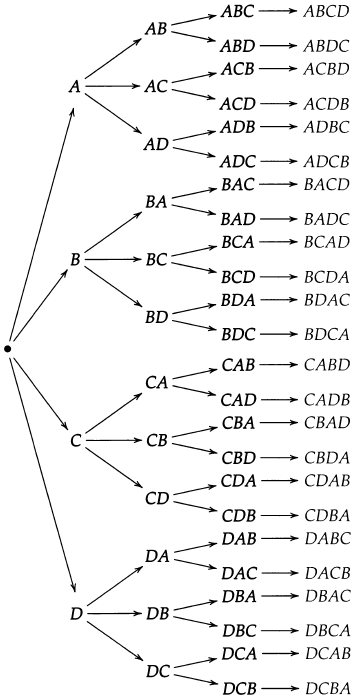
\includegraphics[width=60mm]{1.png}
\caption{Permutations of $ABCD$ visualized}
\end{figure}

The above figure shows how to generate permutations of $ABCD$. We start with 4 choices for the first letter. Once we got the first letter, there are three choices remaining for the second letter and so on.

\begin{texample}
Find the number of words created from rearranging letters $ALLELE$. \\

There are two $E$s and three $L$s. Notice that there is no difference when you reorder these letters. Each word created from two $E$s and three $L$s corresponds to $2!3!$ permutations. \\

The number of permutations is $6!$ which includes duplicates. To get the final answer, we divide it by $2!3!$ which gives $\frac{6!}{2!3!}=60$ total words.
\end{texample}

\begin{texample}
Calculate the probability of obtaining exactly $3$ heads and tails for a total of 6 coin tosses. \\

There are the total of $2^6=64$ possible outcomes. The number of times when the combination $HHHTTT$ occurs is $\frac{6!}{3!3!}=20$. Therefore the probability is $\frac{20}{64}=\frac{5}{16}$.
\end{texample}

To calculate the number of permutations made from choosing $k$ out of $n$ items with no repetition:

$$n(n-1)(n-2) \cdots (n-k+1)=\frac{n!}{(n-k)!}$$

It is usually denoted by ${}_n \mathrm{P}_k$.

\subsection{Combinations}

\begin{texample}
How many ways to pick two out of $\{a, b, c, d\}$? \\

Initially, there are four choices for the first letter of an ordered pair. After picking one, there are three choices left. There are $4(3)=12$ ordered pairs: $ab, ba, ac, ca, ad, da, bc, cb, bd, db, cd, dc$. However, we don't care about the order (ie. $ab$ and $ba$ is considered the same) so we divide by $2!$ which gives: $\frac{12}{2}=6$ combinations.
\end{texample}

To pick $k$ out of $n$ items, the total number of combinations is the number of ways to create ordered combinations (permutations) of size $k$ divided by the number of permutations of $k$ items in combinations. The calculation process is outlined below:

\begin{align*}
\frac{n(n-1)(n-2) \cdots (n-k+1)}{k!} = \frac{\frac{n!}{(n-k)!}}{k!} = \frac{n!}{k!(n-k)!}
\end{align*}

We use $\binom{n}{k}$ to denote $\frac{n!}{k!(n-k)!}$. It is read as ``n choose k.'' This is a binomial coefficient. Another way to think about combinations is that it is the same as finding how many ways to rearrange $n$ cards where $k$ cards are coloured red and $n-k$ cards are coloured green. Also note that:

\begin{align*}
\binom{n}{n-k} = \frac{n!}{(n-k)!(n-(n-k))!} = \frac{n!}{(n-k)!k!} = \binom{n}{k}
\end{align*}

$\binom{n}{k}$ is maximized when $k=n/2$.

\begin{texample}
How many ways to deal $52$ cards to $4$ players? \\

We count the number of ways to pick $13$ cards from the deck of $52$ cards. We then multiply it by the number of ways to pick another set of $13$ cards from the deck of $52-13=39$ cards. We multiply it again by the number of ways to pick another set of $13$ cards from the deck of $39-13=26$ cards. The remaining number of cards is $26-13=13$ which will be given to the last player.

$$\binom{52}{13}\binom{39}{13}\binom{26}{13}\binom{13}{13}=\frac{52!}{(13!)^4}$$
\end{texample}

There is an interesting observation that can be used to calculate binomial coefficients. Suppose you toss a coin $n$ times and $k$ of $n$ tosses are heads. The number of possible ways to get $k$ heads out of $n$ tosses is given by $\binom{n}{k}$. To find this binomial coefficient, consider two cases: the first toss is H and the first toss is not H. When the first toss is H, the remaining tosses $n-1$ must have $k-1$ heads and the number of possible ways it can happen is $\binom{n-1}{k-1}$. When the first toss is not H,  the remaining tosses $n-1$ must have $k$ heads and the number of possible ways it can happen is $\binom{n-1}{k}$. The number of possible ways to get $k$ heads out of $n$ tosses is the number of possible ways to get H as the first toss plus the number of possible ways not to get H as the first toss:

$$\binom{n}{k} = \binom{n-1}{k-1} + \binom{n-1}{k}$$

This is called ``Pascal's rule.'' It can be used to construct Pascal's triangle.

\begin{center}
\begin{tabular}{rccccccccc}
&    &    &    &    &  1\\\noalign{\smallskip\smallskip}
&    &    &    &  1 &    &  1\\\noalign{\smallskip\smallskip}
&    &    &  1 &    &  2 &    &  1\\\noalign{\smallskip\smallskip}
&    &  1 &    &  3 &    &  3 &    &  1\\\noalign{\smallskip\smallskip}
&  1 &    &  4 &    &  6 &    &  4 &    &  1\\\noalign{\smallskip\smallskip}
\end{tabular}
\end{center}

$\binom{n}{k}$ gives the value at $n$th row and $k$th column (both zero-indexed) of the triangle. For example, in the third row and second column, $\binom{2}{1}=2$. Notice that the total in each row is always $2^n$.

\subsection{Multinomial Coefficient}

The binomial coefficient formula $\binom{n}{k}$ can also be thought of as the number of ways to distribute $n$ items into two boxes in such way that one box has $k$ items and the another has $n-k$ items. Multinomial coefficient generalizes this fact to multiple boxes. \\

The formula for the multinomial coefficient can be derived from binomial coefficients. Suppose you have $r$ boxes where you want to distribute (distinct) $n$ items. You want each box to have $k_1, k_2, k_3, \dots, k_r$ items with $k_1+k_2+\cdots + k_r=1$. You first count the number of ways to distribute $k_1$ items in the first box with $n-k_1$ items remaining and this gives $\binom{n}{k_1}$. Then using the remaining $n-k_1$ items to count the number of ways to distribute $k_2$ items in the second box which gives $\binom{n-k_2}{k_2}$. There are $n-k_1-k_2$ items left and this will be used to calculate the number of ways to distribute $k_3$ items into the third box and so on. The number of ways to distribute $n$ items into $m$ boxes is therefore:

\begin{align*}
\binom{n}{k_1}\binom{n-k_1}{k_2}\binom{n-k_1-k_2}{k_3}\ldots\binom{k_{r-1}+k_r}{k_{r-1}}\binom{k_r}{k_r}
\end{align*}

Simplifying this expression gives multinomial coefficient:

\begin{align*}
\boxed{\binom{n}{k_1, k_2, k_3, \dots, k_r} = \frac{n!}{k_1! k_2! k_3! \cdots k_r!}}
\end{align*}

This can also be interpreted as the number of words if letters appear $k_1, k_2, k_3, \dots, k_r$ times. The fourth example can also be solved with $\binom{6}{1, 2, 3}$.

\begin{texample}
How many ways to arrange the sequence of letters $ABRACADABRA$ in such way that there are no consecutive $A$s? \\

The position of $A$s must be five numbers from $\{1, 2, 3, \dots, 11\}$ with no two consecutive numbers. Denote positions of each of the five $A$s by $i,j,k,l,m$ and $i, j-1, k-2, l-3, m-4$ should not contain repetitions. This means $i, j-1, k-2, l-3, m-4$ should take five numbers from $\{1, 2, 3, \dots, 7\}$. There are $\binom{7}{5}=21$ possible sets of locations for the $A$s. For each of them, there are $\binom{6}{4,4}=180$ arrangements for the remaining letters. The overall answer is $21(180)=3780$.
\end{texample}

\subsection{Stars and Bars}

A graphical aid involving stars and bars can solve a wide range of problems. Let's walk over the following examples.

\begin{texample}
There are $5$ buckets of ice cream, each with different flavour. How many ways to make $3$ scoops, provided repetitions are allowed?

It is easier to solve this problem by considering this related problem. We first line up $5$ stars like this:

$$\star\quad \star\quad \star\quad \star\quad \star$$

We then replace a star with $3$ bars:

$$\star\quad \star\quad \star\quad |||\quad \star$$

A star means ``skip'' and a bar means ``serve.'' In this example, the first three ice cream buckets are skipped and all three scoops are from the fourth ice cream bucket. We reduced the original problem is reduced to: ``how many ways to arrange $4$ stars and $3$ bars in $4+3=7$ places?'' This gives $\binom{7}{3}=35$ ways.
\end{texample}

Number of combinations made from choosing $k$ items from $n$ when duplicates are allowed is summarized by the below formula:

$$\binom{n+k-1}{k}$$

\begin{texample}
How many different possible face value combinations created from rolling $3$ dice? \\

This is similar to the ice cream problem we did earlier but with $6$ different ice cream choices. The answer is ${6+3-1 \choose 3}=56$.
\end{texample}

\begin{texample}
How many solutions does the equation $a+b+c=12$ have, where $a,b,c$ are non-negative integers? \\

We first line up $12$ stars like this:

$$\star\quad \star\quad \star\quad \star\quad \star\quad \star\quad \star\quad \star\quad \star\quad \star\quad \star\quad \star$$

We then insert $2$ bars between the stars, for example:

$$\star\quad \star\quad \star\quad |\star\quad \star\quad \star\quad \star\quad |\star\quad \star\quad \star\quad \star\quad \star$$

Here, it represents one solution: $3+4+5=12$. We reduced the original problem is reduced to: ``how many ways to arrange $12$ stars and $2$ bars in $12+2=14$ places?'' The answer is $\binom{14}{2}=91$ solutions.
\end{texample}

\section{Probability}

\subsection{Terminology}

\begin{itemize}
  \item \textbf{Sample space} (denoted by $S$ or $\Omega$): A set of all possible outcomes of an experiment. For example, if an experiment involves rolling a die, its sample space is: $S=\{1, 2, 3, 4, 5, 6\}$. Another example: for an experiment involving drawing a set of five cards from a deck of $52$ cards, its sample space consists of all possible sets of five cards and its size is $|S|=\binom{52}{5}$.
  \item \textbf{Event} (denoted by $E$): An event is any subset of sample space: $E \subset S$. The event $E$ occurs when the outcome of the experiment is a member of $E$. In the dice example, the event would be something like ``number less than 4 appear on the roll'': $E=\{1, 2, 3\}$. In the poker example, $E$ would be a set of outcomes where there is a full house.
\end{itemize}

Consider two events $E_1$ and $E_2$. Union of events $E_1 \cup E_2$ consists of outcomes that are either in $E_1$ or $E_2$ or both. Intersection $E_1 \cap E_2$ consists of outcomes which are both in $E_1$ and $E_2$. Events are said to be disjoint (or mutually exclusive) iff $E_1 \cap E_2 = \emptyset$. The complement of the event $E$ is denoted by $E^c$. It is the set of outcomes in $S$ that is not in $E$. \\

Events follow distributive laws: $E_1 \cap (E_2 \cup E_3) = (E_1 \cap E_2) \cup (E_1 \cap E_3)$ and $E_1 \cup (E_2 \cap E_3) = (E_1 \cup E_2) \cap (E_1 \cup E_3)$. \\

Revisiting the dice example, let $E_1$ be the event when a number less than 4 appears on the roll: $E_1=\{1, 2, 3\}$ and let $E_2$ be the event when an odd number appears on the roll: $E_2=\{1, 3, 5\}$. Union of the these events is: $E_1 \cup E_2 = \{1, 2, 3, 5\}$ and the intersection is: $E_1 \cap E_2 = \{1, 3\}$. The complement of $E_1$ is $E_1^c=\{4, 5, 6\}$.

\begin{figure}[H]
\centering
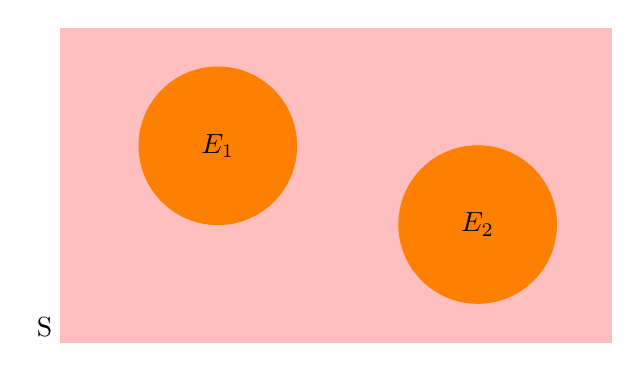
\begin{tikzpicture}
\fill[pink] (0,0) rectangle (7,4);
\draw[orange,fill=orange] (2,2.5) circle (1);
\draw[orange,fill=orange] (5.3,1.5) circle (1);
\node at (-0.2,0.2) {S};
\node at (2,2.5) {$E_1$};
\node at (5.3,1.5) {$E_2$};
\end{tikzpicture}
\caption{Cartoon illustrating sample space $S$ and disjoint events $E_1$ and $E_2$}
\end{figure}

\subsection{Defining Probability}

When repeating the experiment with sample space $S$ $n$ times, let $N_n (E)$ be the number of times $E$ occurs. Probability $P(E)$ of the event $E$ is defined as:

$$\displaystyle P(E) = \lim_{n \to \infty} \frac{N_n (E)}{n}$$

More formally, Probability is defined as a measure which is a function $P$ that assigns to each $E$ as a number and satisfies the following axioms:

\begin{enumerate}[i]
  \item $0 \le P(E) \le 1$ for all $E$
  \item $P(S)=1$ and $P(\emptyset)=0$
  \item For disjoint events $E_1, E_2, ..., E_N$: $\displaystyle P\left( \bigcup_{n=1}^N E_n \right)=\sum_{n=1}^N P(E_n)$
\end{enumerate}

If $S$ is finite (which happens often), we care about finite sequence of events only. The tuple $(S,\mathcal{F},P)$ constructs a probability space where $\mathcal{F}=\mathcal{P}(S)$\footnote{$\mathcal{P}$ is power set} is an event space which consists of all possible outcomes in the sample space $S$. Each event is often equally likely but not always (see the coin-flipping example below for instance). When events are equally likely, $P(E)=\frac{|E|}{|S|}$.

\begin{texample}
A coin is tossed until either two Tails appear successively, or until the fifth toss, whichever comes first. The outcome is the resulting sequence of coins. \\

There are $20$ possible outcomes which is described by the following sample space

\begin{align*}
S&=\{(HHHHH), (THHHH), (HTHHH), (HHTHH), \\
&\quad (HHHTH), (HHHHT), (TT), (HTT), (HHTT), (THTT), \\
&\quad (HHHTT), (THHHT), (HTHHT), (HHTHT), (HHTTH), \\
&\quad (THHTH), (HTHTH), (HTTHH), (THTHH), (TTHHH)\}
\end{align*}

Outcomes in this sample space is not equally likely. For example $P(\{(TT)\})=\frac{1}{4}$ and $P(\{(HTT)\})=\frac{1}{8}$. The total probability is

\begin{align*}
P(S)&=P(\{(TT)\})+P(\{(HTT)\}) \\
&\quad+2 P(\{(HHTT)\})+16  P(\{(HHHTT)\}) \\
&=\frac{1}{4}+\frac{1}{8}+2\frac{1}{16}+16\frac{1}{32} \\
&=1
\end{align*}

as expected.
\end{texample}

\begin{texample}
In the game of poker, find $P(\text{four of a kind})$, $P(\text{full house})$, $P(\text{a pair})$, $P(\text{two pairs})$, and $P(\text{straight})$. \\

As mentioned before, the size of the sample space is $|S|=\binom{52}{5}=2598960$. We need to find how many possible sets of four-of-a-kind $|E|$. There are $13$ different values for the first four cards (there are four suit options and each of the four cards takes a distinct suit but we don't count permutations here) and once the four cards are out, there are $48$ ($12$ choices for value and $4$ choices for suit) options for the last card. So $|E|=13(48)=624$. Therefore, $P(\text{four of kind})=\frac{|E|}{|S|}=0.00024$. \\

There are $13$ possible card values for the first three cards. They can take any suit and there are $\binom{4}{3}=4$ different suit combinations for the first three cards. For the remaining two cards, there are $12$ possible values and $\binom{4}{2}=6$ different suit combinations. So $|E|=3744$ and the probability is therefore $P(\text{full house})=0.00144$. \\

There are $\binom{13}{1}$ ways to pick a value for a pair. There are $\binom{4}{2}$ different suit combinations for a pair. There are $\binom{12}{3}$ ways to pick $3$ distinct values for the rest of the $3$ cards and each card has $\binom{4}{1}$ different suit combinations. The answer is $\frac{\binom{13}{1}\binom{4}{2}\binom{12}{3}\binom{4}{1}^3}{\binom{52}{5}}=0.4226$. \\

There are $\binom{13}{2}$ ways to pick values for two pairs. There are $\binom{4}{2}$ different suit combinations for each pair. There are $\binom{11}{1}$ ways to pick a distinct value for the last card and has $\binom{4}{1}$ different suit combinations. The answer is $\frac{\binom{13}{2}\binom{4}{2}^2\binom{11}{1}\binom{4}{1}}{\binom{52}{5}}=0.04754$. \\

There are 10 possible values for the initial card. There are 4 suit options for each of the five cards, so there are $4^5$ suit combinations but to exclude straight flushes we subtract it by 4. This gives $|E|=10(4^5-4)=10200$, so $P(\text{straight})=0.00392$.
\end{texample}

\begin{texample}
There are $7$ marbles in a bag, $4$ red and $3$ blue. You draw marbles one at a time without replacement. What is the probability that the fifth marble is blue? \\

One way to do this problem is to try labelling each marble from $1$ to $7$ which represents the order of drawing out. So the probability that the blue marble gets $5$ is $\frac37$.
\end{texample}

\begin{texample}
You roll five dice, find probabilities for (a) one pair ($aabcd$) (b) two pairs ($aabbc$) (c) full house ($aaabb$). \\

(a) There are $\binom{6}{4}$ ways to pick values for the set $\{a, b, c, d\}$. There are $\frac{5!}{2!}$ ways to arrange $aabcd$. There are $4$ ways to select the value of a pair from the set $\{a, b, c, d\}$. There are $6^5$ permutations in total. The final answer is $\frac{\binom{6}{4}\frac{5!}{2!}4}{6^5}=0.46296$. \\

(b) Caring about order, there are $\binom{6}{2}$ ways to pick values for the pairs $\{a, b\}$ and $\binom{4}{1}$ ways to pick the value of $c$. There are $\frac{5!}{2!2!}$ ways to arrange $aabbc$. There are $6^5$ permutations in total. The final answer is $\frac{\binom{6}{2}\binom{4}{1}\frac{5!}{2!2!}}{6^5}=0.23148$. \\

(c) There are $\binom{6}{1}$ ways to pick values for $a$ and $\binom{5}{1}$ ways to pick values for $b$. There are $\frac{5!}{3!2!}$ ways to arrange $aaabb$. The final answer is $\frac{\binom{6}{1}\binom{5}{1}\frac{5!}{3!2!}}{6^5}=0.03858$.
\end{texample}

Note on counting: $\binom{6}{1}\binom{5}{1}$ is not equal to $\binom{6}{2}$. The former is used if order matters otherwise the latter is used. In fact, $\binom{6}{1}\binom{5}{1}=2\binom{6}{2}={}_6P_2$. Imagine you have a bag of marbles labelled $1, 2, \dots, 6$, $\binom{6}{2}$ counts the number of two marble combinations while $\binom{6}{1}\binom{5}{1}$ counts the number of ways to pick the first marble and paint it red then pick the second marble.

\begin{texample}
A box contains $15$ lego bricks: $3$ red bricks, $3$ green bricks, $3$ blue bricks, $3$ yellow bricks and $3$ purple bricks. You draw 5 bricks from the box at random without replacement. What is the probability of getting $5$ distinct colours? \\

There are $15\cdot14\cdot13\cdot12\cdot11$ different ordered selections ($15$ options for the first brick, $14$ options for the second brick and so on). Now, there are $15$ options for the first brick which can be in any colour. Then there are $12$ options for the second brick (we exclude all bricks with the same colour as the first brick). There are $9$ options for the third brick (we exclude all bricks with the same colour as the first and second bricks) and so on. The probability is

\[\frac{15}{15}\frac{12}{14}\frac{9}{13}\frac{6}{12}\frac{3}{11}=\frac{81}{1001}\]
\end{texample}

\begin{texample}
You have $13$ cards, $6$ red ($R$) and $7$ black ($B$). You shuffle them and place them face up in two rows. The top row has $5$ cards, the bottom row $8$. If you do this many times, what number of red cards will the top row have most often? \\

The total number of arrangements is $\frac{13!}{6!7!}=1716$. \\

To determine the most likely number of red cards, we count the number of arrangements when the top row has $0, 1, 2, 3, 4, 5$ red cards. For example, to count the number of arrangements for the top row with $2$ red cards, $\binom{5}{2}=\frac{5!}{2!3!}=10$. To get the total number of arrangements we multiply the results, for example, the total number of arrangements with $3$ red cards at the top is $10(56)=560$. After that, we calculate probabilities and compare.

\begin{center}
\footnotesize
\begin{tabular}{l|l|l|l|l|l|l}
  \text{no. red at top} & 0 & 1 & 2 & 3 & 4 & 5 \\
  \hline
  \text{no. arrangements for top} & 1 & 5 & 10 & 10 & 5 & 1 \\
  \hline
  \text{no. red at bottom} & 6 & 5 & 4 & 3 & 2 & 1 \\
  \hline
  \text{no. arrangements for bottom} & 28 & 56 & 70 & 56 & 28 & 8 \\
  \hline
  \text{total no. of arrangements} & 28 & 280 & 700 & 560 & 140 & 8 \\
  \hline
  \text{probability} & 0.016 & 0.163 & 0.408 & 0.326 & 0.082 & 0.005
\end{tabular}
\end{center}

From the table, we see that the top row will most likely have $2$ red cards. \\

Also notice that $28+280+700+560+140+8=1716$. \\

If we were to compute the average number of red cards in the top row, we use the following relation: $\sum_{n=0}^5 nP_n$ where $P_n$ is the probability of getting $n$ red cards in the top row. This gives:

$$0(0.016) + 1(0.163) + 2(0.408) + 3(0.326) + 4(0.082) + 5(0.005)=2.31$$

This playing card example has applications in statistical mechanics for modelling two-state systems.
\end{texample}

\begin{texample}
You have a standard deck of $52$ cards which consists of $26$ red cards and $26$ black cards. The deck is shuffled well, what is the probability that the first five cards contain $3$ red cards and $2$ black cards? What is the probability if the deck is large enough? \\

We count the number of ways to draw $3$ red cards from the set of $26$ red cards: $\binom{26}{3}$ and the number of ways to draw $2$ black cards from the set of $26$ black cards: $\binom{26}{2}$. Then multiply the result and divide it by the number of ways to draw $5$ cards from the deck: $\binom{52}{5}$. This gives $P(3R,2B)=\frac{\binom{26}{3}\binom{26}{2}}{\binom{52}{5}}$. \\

Alternative approach: Count the number of combinations of a $5$ card hand that contains $3$ red and $2$ black: $\binom{5}{3}$. Then count the number of ways to rearrange the remaining cards in the deck: $\binom{52-5}{26-3}$. Finally count the number of ways to arrange the deck: $\binom{52}{26}$. This gives $P(3R,2B)=\frac{\binom{5}{3}\binom{52-5}{26-3}}{\binom{52}{26}}$. \\

To approximate the probability when the deck is large, we rewrite things a bit:

\begin{align*}
P(3R,2B)&=\frac{\binom{26}{3}\binom{26}{2}}{\binom{52}{5}} \\
&=\frac{\frac{26!}{3!23!}\frac{26!}{2!24!}}{\frac{52!}{5!47!}} \\
&=\frac{5!}{3!2!}\frac{\frac{47!}{23!24!}}{\frac{52!}{26!26!}} \\
&=\frac{5!}{3!2!}\frac{(52-5)!26!26!}{52!(26-3)!(26-2)!} \\
&=\frac{5!}{3!2!}\frac{26(26-1)(26-2)26(26-1)}{52(52-1)(52-2)(52-3)(52-4)} \\
&\approx \frac{5!}{3!2!}\frac{26^5}{56^5} \\
&\approx \frac{5!}{3!2!}\frac{1}{2^5}
\end{align*}

We conclude that the suitable approximation is $\frac{\binom{5}{3}}{2^5}$. This gets better when the deck is larger. \\

This example illustrates the concept of heat bath. The larger the deck is, taking out a few cards will have almost no effect on the probability.
\end{texample}

\subsection{Useful Probability Relations}

Probability has the following useful properties:

\begin{enumerate}[i]
  \item For a single event $E$, $P(S)=P(E)+P(E^c)=1$. $E$ and $E^c$ is always disjoint.
\begin{figure}[H]
\centering
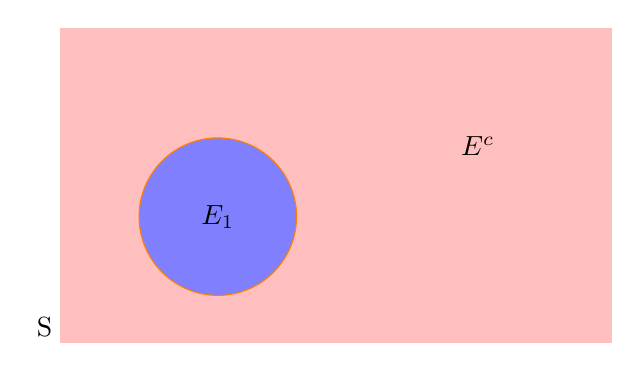
\begin{tikzpicture}
\fill[pink] (0,0) rectangle (7,4);
\draw[orange,fill=blue!50] (2,1.6) circle (1);
\node at (-0.2,0.2) {S};
\node at (2,1.6) {$E_1$};
\node at (5.3,2.5) {$E^c$};
\end{tikzpicture}
\caption{Event $E$ and its complement $E^c$}
\end{figure}
  \item For two non-disjoint events $E_1$ and $E_2$, probability can be calculated using inclusion-exclusion principle: $P(E_1 \cup E_2) = P(E_1) + P(E_2) - P(E_1 \cap E_2)$.
\def\firstcircle{(0,0) circle (1.8cm)}
\def\secondcircle{(0:2cm) circle (1.8cm)}
\begin{figure}[H]
\centering
\begin{tikzpicture}
\begin{scope}[shift={(3cm,-5cm)}, fill opacity=0.5]
    \fill[pink] (-3,-2.3) rectangle (5,2.3);
    \fill[red] \firstcircle;
    \fill[green] \secondcircle;
    \draw \firstcircle node [left] {$E_1$};
    \draw \secondcircle node [right] {$E_2$};
    \node at (0:1cm) {$E_2 \cap E_2$};
    \node at (-3.2,-2.2) {S};
\end{scope}
\end{tikzpicture}
\caption{Cartoon illustrating non-disjoint events $E_1$ and $E_2$}
\end{figure}
For disjoint events, $P(E_1 \cap E_2)$ = 0 since $E_1 \cap E_2 = \emptyset$. \\

For three events, it becomes:

\begin{align*}
P(E_1 \cup E_2 \cup E_3) &= P(E_1) + P(E_2) + P(E_3) \\
&\phantom{-} - P(E_1 \cap E_2) - P(E_2 \cap E_3) - P(E_1 \cap E_3) \\
&\phantom{-} + P(E_1 \cap E_2 \cap E_3)
\end{align*}

\begin{figure}[H]
\centering
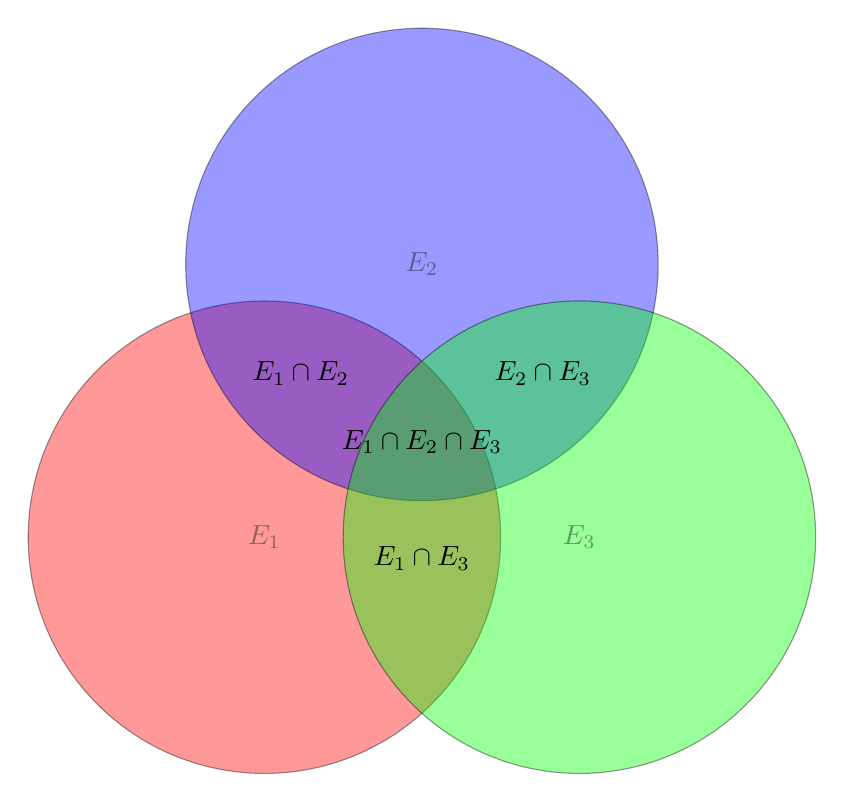
\begin{tikzpicture}
  \tikzset{venn circle/.style={draw,circle,minimum width=6cm,fill=#1,opacity=0.4}}
  \node [venn circle = red] (A) at (0,0) {$E_1$};
  \node [venn circle = blue] (B) at (60:4cm) {$E_2$};
  \node [venn circle = green] (C) at (0:4cm) {$E_3$};
  \node[left] at (barycentric cs:A=1/2,B=3/4 ) {$E_1 \cap E_2$}; 
  \node[below] at (barycentric cs:A=1/2,C=1/2 ) {$E_1 \cap E_3$};   
  \node[right] at (barycentric cs:B=3/4,C=1/2 ) {$E_2 \cap E_3$};   
  \node[below] at (barycentric cs:A=1/3,B=1/2,C=1/3 ){$E_1 \cap E_2 \cap E_3$};
\end{tikzpicture}  
\caption{Three non-disjoint events $E_1$, $E_2$ and $E_3$}
\end{figure}

For more than three events, the inclusion-exclusion principle can be generalized to:

\begin{align*}
P\left( \bigcup_{n=1}^N E_n \right) &= \sum_{i} P(E_i) \\
&\phantom{-} - \sum_{i<j} P(E_i \cap E_j) \\
&\phantom{-} + \sum_{i<j<k} P(E_i \cap E_j \cap E_k) \\
&\phantom{-} - \sum_{i<j<k<l} P(E_i \cap E_j \cap E_k \cap E_l) + \cdots + (-1)^{n-1} P\left( \bigcap_{n=1}^N E_n \right)
\end{align*}
\end{enumerate}

\begin{texample}
Birthday problem: There are $n$ people in the room, what is the probability that at least two of them share the same birthday? \\

The sample space $S$ for this experiment consists of sequences of $n$ birthdays: $(B_1, B_2, \dots, B_n) \in S$. The size of the sample space is $|S|=365^n$, ignoring leap years. The event $E$ is the set of sequences that contains at least two matching birthdays, like for example $E=\{\dots (09/11, \dots, 09/11) \dots\}$. \\

We first calculate the probability that all $n$ birthdays are different. This is the complement of the event $E$, denoted by $E^c$. There are $365$ unique choices for the first person's birthday and this leaves with $364$ choices for the second person's birthday and so on. The probability is:

$$ P(\text{all different})=\frac{|E^c|}{|S|}=\frac{365 \cdot 364 \cdot 363 \cdots (365-n+1)}{365^n}=\frac{{}_{365} \mathrm{P}_n}{365^n}$$

The probability that at least two people share the same birthday is therefore:

$$P(\text{at least two same bday})=1-P(\text{all different})=1-\frac{{}_{365} \mathrm{P}_n}{365^n}$$

To illustrate the result, suppose $n=23$, the probability is $P(\text{at least two same bday})=0.5073$.
\end{texample}

\begin{texample}
You flip two coins. Find the probability that either the first or the second coin fall heads. \\

The possible outcomes $S$ for this experiment are: $S=\{(H, H), (H, T), (T, H), (T,T)\}$. Let $E_1$ be the event that the first coin falls heads: $E_1=\{(H, H), (H, T)\}$ and $E_2$ be the event that the second
coin falls heads: $E_2=\{(H, H), (T, H)\}$. By the inclusion-exclusion principle:

\begin{align*}
P(E_1 \cup E_2) &= P(E_1) + P(E_2) - P(E_1 \cap E_2) \\
&= \frac{1}{2}+\frac{1}{2}-\frac{1}{4}=\frac{3}{4}
\end{align*}

It can be computed directly as well: $P(E_1 \cup E_2)=P(\{(H, H), (H, T), (T, H)\})=\frac{3}{4}$.
\end{texample}

\begin{texample}
Find the probability that the random permutation of $1112345$ does not have adjacent identical digits. \\

We label $1$s to distinguish them: $1_a 1_b 1_c 2345$. The sample space $S$ is all permutations of $1_a 1_b 1_c 2345$ and the size is $|S|=7!=5040$ (remember that $1$s are distinct from each other!). Let $E_{ab}$, $E_{bc}$, $E_{ac}$ denote events where ``$1_a$ and $1_b$ are adjacent,'' ``$1_b$ and $1_c$ are adjacent'' and ``$1_a$ and $1_c$ are adjacent'' respectively. The probability that there are no adjacent ones can be calculated using the inclusion-exclusion principle:

\begin{align*}
P(\text{no adjacent 1s}) &= 1 - P(E_{ab} \text{ or } E_{bc} \text{ or } E_{ac}) \\
&= 1 - P(E_{ab}) - P(E_{bc}) - P(E_{ac}) \\
& \quad + P(E_{ab} \text{ and } E_{bc}) + P(E_{ab} \text{ and } E_{bc})  \\
& \quad + P(E_{ac} \text{ and } E_{bc}) \\
& \quad - P(E_{ab} \text{ and } E_{bc} \text{ and } E_{ac})
\end{align*}

By symmetry and the fact that $1_a, 1_b, 1_c$ cannot *all* be adjacent to each other:

$$P(\text{no adjacent 1s}) = 1 - 3 P(E_{ab}) + 3 P(E_{ab} \text{ and } E_{bc})$$

$P(E_{ab}) = \frac{2 (6!)}{7!} = \frac27$: if $1_a$ and $1_b$ are adjacent, we can treat them as one symbol $[1_a 1_b]$, so there are $6!$ ways to order the $6$ symbols we now have, and then $2$ ways to choose the order of $1_a$ and $1_b$. Similarly, $P(E_{ab} \text{ and } E_{bc})$ can be calculated by treating $[1_a 1_b 1_c]$ as a symbol. There are two valid permutations where $[1_a 1_b]$ and $[1_b 1_c]$ combinations exist, namely $[1_a 1_b 1_c]$ and $[1_c 1_b 1_a]$. This gives $\frac{2 (5!)}{7!}=\frac{1}{21}$. \\

The final answer is:

$$P(\text{no adjacent 1s}) = 1 - 3 \frac27 + 3 \frac{1}{21} = \frac27$$
\end{texample}

\begin{texample}
$n$ people put their names in a hat. The hat is shaken and $n$ people draw names out of the hat (secret Santa). What is the probability that nobody gets their own name? \\

We label each person from $1$ to $n$. The sample space $S$ is all permutations of $\{1, 2, \dots, n\}$ and its size is $|S|=n!$. Let $E_i$ denote an event where person $i$ gets their own name: $E_i=\{ \text{permutations where person $i$ gets their own name.} \}$. We first calculate $P(E_1 \cup E_2 \cup \cdots \cup E_n)$. \\

First, we calculate $P(E_i)$. The number of events where person $1$ gets his own name $|E_1|$ can be calculated by placing person $1$ on position $1$ from the start and counting the number of ways to arrange the remaining $n-1$ people on positions $2, 3, \dots n$ which is $(n-1)!$. The probability that person $1$ gets his own name is $P(E_1)=\frac{(n-1)!}{n!}=\frac{1}{n}$. By symmetry, $P(E_i)=P(E_1)$ for $i=1, 2, \dots n$. \\

Next we calculate $P(E_i \cap E_j)$. $|E_1 \cap E_2|$ is the number of events where both person $1$ and person $2$ gets their own names. The calculation process is similar: place persons $1$ and $2$ at positions $1$ and $2$ respectively and calculate the number of ways to arrange the remaining $n-2$ people on positions $3, \dots n$ which is $(n-2)!$. So, $P(E_1 \cap E_2)=\frac{(n-2)!}{n!}$ and by symmetry, $P(E_i \cap E_j)=P(E_1 \cap E_2)$ for any $i<j$. There are $\binom{n}{2}$ pairs of $i,j$. \\

We can generalize that the probability that $k$ people get their own names is $\frac{(n-k)!}{n!}$ and there are $\binom{n}{k}$ combinations of $k$ people. Now by the inclusion-exclusion principle:

\begin{align*}
P\left( \bigcup_{n=1}^N E_n \right) &= n P(E_1) - \binom{n}{2} P(E_1 \cap E_2) + \binom{n}{3} P(E_1 \cap E_2 \cap E_3) \\
&\phantom{-} + \cdots \pm (-1)^{n-1} P\left( \bigcap_{n=1}^N E_n \right) \\
&= n\frac{1}{n} - \binom{n}{2}\frac{(n-2)!}{n!} + \binom{n}{3}\frac{(n-3)!}{n!} - \dots + \frac{(-1)^{n-1}}{n!} \\
&= \sum_{k=1}^N (-1)^{k-1}\binom{n}{k}\frac{(n-k)!}{n!} \\
&= \sum_{k=1}^N (-1)^{k-1} \frac{1}{k!} = 1-e^{-1}
\end{align*}

Therefore the probability that nobody draws their own name is $1-(1-e^{-1})=e^{-1}=0.368$.
\end{texample}

\subsection{Conditional Probability and Independent Events}

Suppose there are two events $E$ and $F$. Assume that $P(F)>0$. The probability that $E$ happens given that $F$ happened is denoted by $P(E|F)$. Imagine $E$ and $F$ lie on s sample space $S$.

\def\firstcircle{(0,0) circle (1.8cm)}
\def\secondcircle{(0:2cm) circle (1.8cm)}
\begin{figure}[H]
\centering
\begin{tikzpicture}
\begin{scope}[shift={(3cm,-5cm)}, fill opacity=0.5]
    \fill[white] (-3,-2.3) rectangle (5,2.3);
    \fill[red] \firstcircle;
    \fill[blue] \secondcircle;
    \draw \firstcircle node [left] {$E$};
    \draw \secondcircle node [right] {$F$};
    \node at (0:1cm) {$E \cap F$};
    \node at (-3.2,-2.2) {S};
\end{scope}
\end{tikzpicture}
\caption{Events $E$ and $F$}
\end{figure}

Recall that the probability of $P(E)$ is proportional to the probability of the sample space $P(S)=1$. When event $F$ happens, $F$ will become a new sample space as illustrated below.

\begin{figure}[H]
\centering
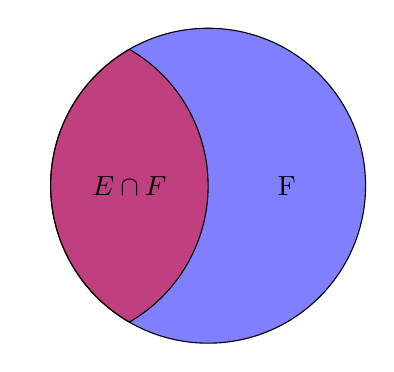
\begin{tikzpicture}
    \draw[fill=blue, fill opacity=0.5] (0,0) circle (2);
    \draw[fill=red, fill opacity=0.5] (120:2)
        arc[start angle=60, end angle=-60, radius=2]
        arc[start angle=240, end angle=120, radius=2];
    \node at (180:1) {$E \cap F$};
    \node at (0:1) {F};
\end{tikzpicture}
\caption{New sample space $F$}
\end{figure}

With this new sample space, we can be sure that everything happens on $F$. $E|F$ indicates both events $E$ and $F$ happen, so we have $E \cap F$ lie in $F$. We can now define $P(E|F)$ as a ratio of $E \cap F$ to $F$, assuming that every outcome in $F$ is equally likely:

$$P(E|F)=\frac{|E \cap F|}{|F|}$$

Dividing both numerator and denominator by $|S|$ gives:

$$P(E|F)=\frac{\frac{|E \cap F|}{|S|}}{\frac{|F|}{|S|}}=\frac{P(E \cap F)}{P(F)}$$

We derived the formula for conditional probability. It satisfies all probability axioms. As a corollary, this formula is also written in this way:

$$P(E \cap F)=P(F)P(E|F)$$

This is intuitive: ``probability for both $E$ and $F$ happen is the probability that $F$ happens times the probability that $E$ happens \textit{given} that $F$ happened.'' \\

Two events $E$ and $F$ are independent if finding out one event does not affect the probability of another, that is $P(E|F)=P(E)$. This means uncovering the existence of $F$ does not affect the probability of $E$ happening. We can test whether events are independent or not using the below relation:

$$P(E \cap F)=P(F)P(E)$$

Note that disjoint and independent are two different things. Events being disjoint means they are mutually exclusive. Here are some examples of (non-)disjoint and (in)dependent events.

\begin{enumerate}
  \item \textbf{Disjoint but dependent events}

Consider an experiment of rolling a die. Define events $E$ to be ``roll $3$'' and $F$ to be ``roll $4$.'' These events are disjoint because you can't roll both $3$ and $4$ at the same time using a single dice and this makes $P(E \cap F)=0$. It implies that events are not independent (ie. dependent) because of $P(E \cap F) \ne P(E)P(F)$. Also since $P(E \cap F)=0$, $P(E|F)=0$ which makes sense in this context. \\ 

We can conclude that disjoint events cannot be independent. There are exceptions, for example, consider the game of darts. Define events $E$ "dart land on target" and $F$ "dart land on the edge of the board." $P(E\cap F)=0$ since a dart land at both places same time but $P(E)=0$ and $P(F)=0$ since there are infinitely many points but it is still possible to land on one of them. Events $E$ and $F$ are disjoint but independent events.
  \item \textbf{Independent but not disjoint events}

Consider the dice experiment again but with two dice this time. Define events $E$ "the sum of the face values is $7$" and $F$ the face value of the first die is $2$. They are not disjoint because there is a possible outcome where the sum of the face value is $7$ and the face value of the first die is $2$: $\{2, 5\}$. $E$ and $F$ are independent because $P(E\cap F)=\frac{1}{36}$ and $P(E)P(F)=\frac{1}{36}$. But if we redefine $E$ to be ``the sum of the face values is $6$,'' the events will become dependent because the probability depends on whether we rolled $6$ on the first roll or not (we must roll numbers $1$ to $5$ to get some chance that the face values totalling $6$).
  \item \textbf{Dependent but not disjoint events}

We discussed an example of dependent but not disjoint events previously but here is another one: In an experiment where you draw two balls from a bag containing $5$ red balls and $3$ green balls without replacement, define events $E$ "draw a red ball on the first draw" and $F$ "two balls are red." They are not disjoint because there is an outcome where $E$ and $F$ happen at the same time: $\{R, R\}$. They are dependent (ie. not independent) because $P(E\cap F)=P(E)P(F|E)=\frac58 \frac47=\frac{5}{14}$ and $P(E)P(F)=\frac58 \frac{5}{14}=\frac{25}{112}$.
\end{enumerate}

For more than two events, events $E_1, E_2, \dots, E_n$ are independent iff

$$P\left(\bigcup_i^k E_{i'} \right) = \prod_i^k P(E_{i'})$$

for every subset $E_{1'}, E_{2'}, \dots. E_{k'}$ of size $k\le n$. \\

If events $A,B,C,D$ are dependent:

$$P(A\cap B\cap C\cap D) = P(A)P(B|A)P(C|A\cap B)P(D|A\cap B\cap C)$$

\begin{texample}
You draw two cards from a standard deck. Define events $E$ ``draw hearts as the first card'' and $F$ ``draw hearts as the second card.'' Find $P(\text{draw two hearts})$. \\

We have $P(E)=P(F)=\frac{13}{52}$ and

$$P(E \cap F)=P(E)P(F|E)=\frac{13}{52}\frac{12}{51}=\frac{1}{17}$$

or alternatively, $P(E \cap F)=\frac{{13 \choose 2}}{{52 \choose 2}}=\frac{1}{17}$. \\

The events $E$ and $F$ are dependent because $P(E \cap F) \ne P(E)P(F)$.
\end{texample}

\begin{texample}
You draw a card from a standard deck. Define events $E$ ``draw red card'' and $F$ ``draw ace.'' Find $P(\text{red ace})$. \\

We find that $P(E)=\frac{1}{2}$ and $P(F)=\frac{4}{52}=\frac{1}{13}$. To find $P(\text{red ace})$, we calculate $P(E \cap F)$:

$$P(E \cap F)=P(F)P(E|F)=\frac{1}{13}\frac{1}{2}=\frac{1}{26}$$

Notice that $P(E|F)=P(E)$ which makes events $E$ and $F$ independent.
\end{texample}

\begin{texample}
You toss two coins. Define events $E$ ``first coin heads,'' $F$ ``second coin heads'' and $G$ ``both heads or both tails.'' Are these three events mutually independent? \\

The sample space is $S=\{HH, HT, TH, TT\}$. We have $P(E)=\frac12$, $P(F)=\frac12$ and $P(G)=\frac12$. Any of these two events are independent, for example, $P(E\cap F)=\frac14$ which is equal to $P(E)P(F)=\frac12\frac12=\frac14$. However, $P(E \cap F \cap G)=\frac14$ which is not equal to $P(E)P(F)P(G)=\frac18$, so the three events combined are not independent.
\end{texample}

\begin{texample}
You roll two dice blindfolded. You are told that the sum is not greater than $3$, what is the probability that both dice have the same face value? \\

Let $E$ be the event when both dice have the same face value and $F$ be the event when the sum is not greater than $3$. Since they both share the $\{1, 1\}$ outcome, the events are not disjoint. \\

We wish to calculate $P(E|F)$. We have $P(E)=\frac{6}{36}=\frac16$ and $P(F)=\frac{3}{36}=\frac{1}{12}$ (the possible outcomes are $\{1, 1\}$, $\{1, 2\}$ and $\{2, 1\}$). The probability to get both events is $P(E \cap F)=\frac{1}{36}$. This makes events $E$ and $F$ dependent since $P(E \cap F) \ne P(E)P(F)$. Therefore $P(E|F)$ is given by:

$$P(E|F)=\frac{P(E \cap F)}{P(F)}=\frac{\frac{1}{36}}{\frac{1}{12}}=\frac{1}{3}$$
\end{texample}

\subsection{Law of Total Probability}

Let $F_1, F_2, \dots, F_n$ denote partitions of sample space $S$ in such way that

$$S=\bigcup_i^n F_i$$

There is also an event $E$ in $S$. We want to find the relationship between $E$ and $F_1, F_2, \dots, F_n$.

\begin{figure}[H]
\centering
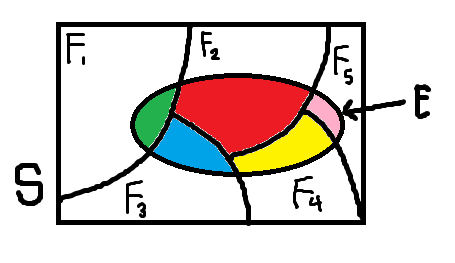
\includegraphics[width=130mm]{2.png}
\caption{Partitions of $S$}
\end{figure}

From the diagram, we see that $E$ is expressed as disjoint unions (coloured regions) of $E \cap F_i$, so

$$P(E)=\sum_i P(E \cap F_i) = \sum_i P(F_i) P(E|F_i)$$

This is the law of total probability. It expresses $P(E)$ in terms of weighted averages of $P(E|F_i)$s. For two events $E$ and $F$ (see figure 6), $E$ can be expressed as $(E\cap F) \cup (E\cap F^c)$ and the law becomes:

\begin{align*}
P(E)&=P(E \cap F)+P(E \cap F^c) \\
&=P(F) P(E|F) + P(F^c) P(E|F^c) \\
&=P(F) P(E|F) + (1-P(F)) P(E|F^c)
\end{align*}

\begin{texample}
You choose a random number from $1$ to $10$ and then you throw that many dice. Define events $E$ ``sum of the face values is $3$'' and $F_i$ ``choose $i$.'' Find $P(E)$. \\

We have $P(F_i)=\frac{1}{10}$ for all $i$ and $P(E|F_1)=\frac16$ (given that we selected $1$, we need to roll $3$ to get the desired sum), $P(E|F_2)=\frac{2}{36}$ (there are two outcomes that give the desired sum: $\{1,2\}$ and $\{2,1\}$) and $P(E_3)=\frac{1}{6^3}$ (the only possible outcome is $\{1,1,1\}$). For $i>3$, achieving the desired sum is impossible at this point so $P(E|F_i)=0$. Now $P(E)$ can be computed as follows:

\begin{align*}
P(E)&=\sum_{i=1}^{10} P(F_i) P(E|F_i) \\
&=P(F_1)P(E|F_1)+P(F_2)P(E|F_2)+P(F_3)P(E|F_3) \\
&\quad +P(F_4)P(E|F_4)+\cdots+P(F_{10})P(E|F_{10}) \\
&=\frac{1}{10}\frac16 + \frac{1}{10}\frac{2}{36}+\frac{1}{10}\frac{1}{6^3}+\frac{1}{10}0+\cdots+0 \\
&=\frac{49}{2160}
\end{align*}
\end{texample}

\subsection{Bayes' Theorem}

For events $E$ and $F$, we found that

$$P(E \cap F)=P(F)P(E|F)$$

but $P(E \cap F)$ can also be calculated in terms of $P(E)$ which gives:

$$P(E \cap F)=P(E)P(F|E)$$

Combining these equations gives:

$$\boxed{P(F|E)=\frac{P(E|F)P(F)}{P(E)}}$$

The formula expressing the relationship between $P(E|F)$ and $P(F|E)$ is known as Bayes' theorem. This powerful relationship has many real-world applications like detecting false positives in medical diagnosis. Once you know $P(E|F)$, $P(E)$ and $P(F)$, then it will be easy to find $P(F|E)$.

\begin{figure}[H]
\centering
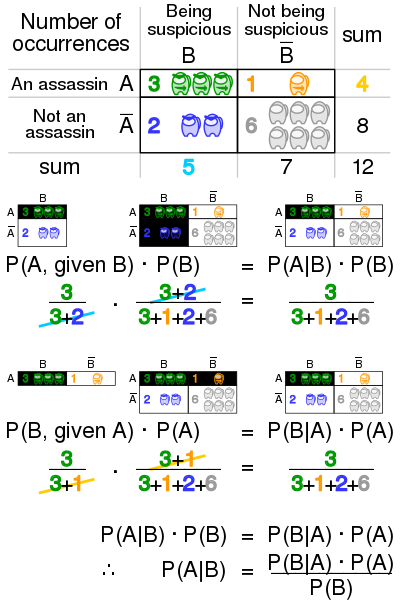
\includegraphics[width=100mm]{3.png}
\caption{Geometric interpretation of Bayes' theorem using Amogus}
\end{figure}

If we apply the law of total probability we derived from the previous section to $P(E)$:

$$P(F|E)=\frac{P(E|F)P(F)}{P(F) P(E|F) + P(F^c) P(E|F^c)}$$

For multiple events $F_1, F_2, \dots, F_n$, it becomes:

$$P(F_j|E)=\frac{P(E|F_j)P(F)}{\sum_i P(E|F_i) P(F_i)}$$

This is useful if we want to determine which one of $F_j$ occurred given that event $E$ happened.

\begin{texample}
Continuing from the last example, what is the probability that you selected $2$ given that the sum is $3$? \\

\begin{align*}
P(F_2|E)&=\frac{P(E|F_2)P(F_2)}{P(F_1)P(E|F_1)+P(F_2)P(E|F_2)+P(F_3)P(E|F_3)} \\
&=\frac{\frac{2}{36}\frac{1}{10}}{\frac{1}{10}\frac16 + \frac{1}{10}\frac{2}{36}+\frac{1}{10}\frac{1}{6^3}}=\frac{12}{49}
\end{align*}
\end{texample}

\begin{texample}
A medical test is carried out to test whether a person has cancer or not. The test is $95\%$ effective at detecting whether the person has cancer or not when it is actually present. However, there is $1\%$ percent of chance of false positive. False positives happen when the test gives a positive result even though the person is perfectly healthy. False negatives happen when the test gives a negative result even though the person actually has cancer. We know that about one in a hundred people have cancer. Find the probability that a person has cancer given that the test gives a positive result. \\

Define events $E$ ``test results in positive,'' $H$ ``person is healthy'' and $C$ ``person has cancer.'' \\

From the description, we know that $P(C)=\frac{1}{100}$, $P(E|C)=\frac{95}{100}$ and $P(E|H)=\frac{1}{100}$. We can infer that $P(H)=1-P(C)=\frac{99}{100}$, $P(\text{false positive})=P(E|H)=\frac{1}{100}$, and $P(\text{false negative})=1-P(E|C)=\frac{5}{100}$. \\

We want to find $P(C|E)$ and it is calculated as follows:

\begin{align*}
P(C|E)&=\frac{P(E|C)P(C)}{P(E)} \\
&=\frac{P(E|C)P(C)}{P(C)P(E|C)+P(H)P(E|H)} \\
&=\frac{\frac{95}{100}\frac{1}{100}}{\frac{1}{100}\frac{95}{100}+\frac{99}{100}\frac{1}{100}} \approx 0.49
\end{align*}
\end{texample}

\begin{texample}
Monty Hall problem: The host puts a prize in one of the three doors. You choose door 1. The host then reveals door 2 which contains no prize. Should you make a switch to door 3? \\

Let $E$ be an event when the host opens door 2 which contains no prize (he can also open other doors not just this door) and $F_i$ be an event when the prize is located in door $i$. \\

Since we don't know which door the prize is in, $P(F_1)=P(F_2)=P(F_3)=\frac13$. The probability that the host will open door 1 is $P(E|F_1)=\frac12$ because he can either open door 2 or door 3 in this case. $P(E|F_2)=0$ because there is no way he would reveal the prize door. $P(E|F_3)=1$ because door 2 is the only door he can open in this case. \\

We want to find $P(F_1|E)$ and $P(F_3|E)$. By Bayes' theorem, we get

$$P(F_1|E)=\frac{P(E|F_1)P(F_1)}{\sum_{j=1}^3 P(E|F_j)P(F_j)}=\frac{\frac12\frac13}{\frac12\frac13+0\frac13+1\frac13}=\frac13$$

and

$$P(F_2|E)=\frac{P(E|F_2)P(F_2)}{\sum_{j=1}^3 P(E|F_j)P(F_j)}=\frac{1\frac13}{\frac12\frac13+0\frac13+1\frac13}=\frac23$$

We definitely should make a switch!
\end{texample}

\section{Random Variables}

\subsection{Introduction}

A random variable is a function that maps elements from a sample space to any real number: $X : S\to\mathbb{R}$. It is usually denoted by $X, Y, Z, N$. Let $s$ be a member of a sample space $S$, if $s$ is picked up by probability function $P$ then random variable $X(s)$ returns a real number. A random variable can either be discrete or continuous. \\

A discrete random variable only takes finite (or countably infinite) $m$ values: $\{x_1, x_2, \dots, x_m\}$. The sample space is broken into discrete partitions.

\begin{figure}[H]
\centering
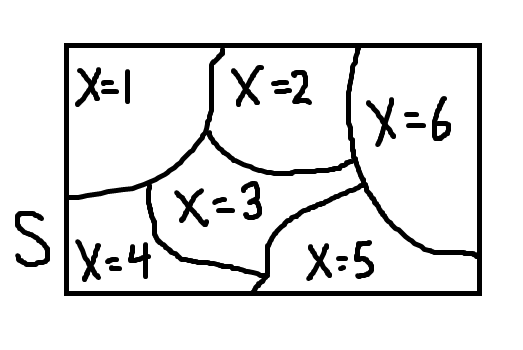
\includegraphics[width=120mm]{4.png}
\caption{Example of a discrete R.V.}
\end{figure}

On the other hand, a continuous random variable can take infinitely many values. One such example is a coordinate on the x-axis which is represented by a real number: $X(x)=x$. \\

The probability when a random variable takes a certain value is denoted by $P(X=a)$ which is the shortcut for writing $P(\{s \in S \mid X(s)=a\})$. Ranges are also allowed: $P(X\le a)=P(\{s \in S \mid X(s)\le a\})$.

\begin{texample}
You roll two dice. Find probabilities of each sum. What is the probability of rolling $30$ or $\pi$? \\

The sample space for two dice rolls is $S=\{(a,b) \mid a,b \in \{1, 2, \dots, 6\}\}$. The random variable relevant to this problem is $X((a,b))=a+b$. Below are probabilities for each possible sum.

\begin{align*}
&P(X = 2) = P((1, 1)) = \frac{1}{36} \\
&P(X = 3) = P((1, 2), (2, 1)) = \frac{2}{36} \\
&P(X = 4) = P((1, 3), (2, 2), (3, 1)) = \frac{3}{36} \\
&P(X = 5) = P((1, 4), (2, 3), (3, 2), (4, 1)) = \frac{4}{36} \\
&P(X = 6) = P((1, 5), (2, 4), (3, 3), (4, 2), (5, 1)) = \frac{5}{36} \\
&P(X = 7) = P((1, 6), (2, 5), (3, 4), (4, 3), (5, 2), (6, 1)) = \frac{6}{36} \\
&P(X = 8) = P((2, 6), (3, 5), (4, 4), (5, 3), (6, 2)) = \frac{5}{36} \\
&P(X = 9) = P((3, 6), (4, 5), (5, 4), (6, 3)) = \frac{4}{36} \\
&P(X = 10) = P((4, 6), (5, 5), (6, 4)) = \frac{3}{36} \\
&P(X = 11) = P((5, 6), (6, 5)) = \frac{2}{36} \\
&P(X = 12) = P((6, 6)) = \frac{1}{36}
\end{align*}

Notice that the total probability adds up to one

$$\sum_{n=2}^{12} P(X=n)=1$$

As for $30$ and $\pi$, the probability is zero.
\end{texample}

\subsubsection{Commutative Distribution Function}

We conclude this section with brief words on commutative distribution functions (CDF). CDF for a random variable $X$ is defined as

$$F_X (a)=P(X\le a)$$

for all $a$ values. In other words, $F_X(a)$ is the sum of probabilities from $-\infty$ to $a$. \\

The basic properties of $F_X(a)$ are:

\begin{enumerate}[i]
  \item $0 \le F_X(a) \le 1$
  \item $F_X(a_1) \le F_X(a_2)$ for $a_1 < a_2$
  \item $\displaystyle \lim_{a\to-\infty} F_X(a)=0$
  \item $\displaystyle \lim_{a\to\infty} F_X(a)=1$
\end{enumerate}

The last two properties indicate the function $F_X(a)$ is monotone increasing. \\

We can calculate probabilities from CDFs using the following relations:

\begin{enumerate}[i]
  \item $P(a<X\le b)=F_X(b)-F_X(a)$
  \item $P(X>a)=1-F_X(a)$
\end{enumerate}

Notice that the first property vaguely resembles the fundamental theorem of calculus. We will see later that CDFs are what we get when we integrate probability density functions (PDF). \\

\subsection{Discrete Random Variables}

Since discrete random variables take a finite number of values, their CDF $F_X(a)$ changes in discrete steps for each value and are constant between jumps (think of stairs). Before we go further, we need to discuss probability mass functions (PMF) first.

\subsubsection{Probability Mass Function}

PMFs $p_X(x)$ are like bar charts used for calculating probability involving discrete random variables. They are defined in such a way that

$$p_X(a)=P(X=a)$$

for a discrete random variable $X$ which takes the following values: $\{x_1, x_2, \dots, x_m\}$. They satisfy the following properties:

\begin{enumerate}[i]
  \item $p_X (x_i) \ge 0$ for all $i$
  \item $\sum_i^m p_X (x_i)=1$
\end{enumerate}

$F_X(a)$ for a discrete variable can be found using: $F_X(a)=P(X\le a)=\sum_{x_i\le a} p_X(x_i)$. \\

We either use $p_X (x)$ or $F_X (a)$ to specify a discrete random variable. We will take a look at some special discrete random variables.

\subsubsection{Bernoulli Random Variable}

Bernoulli random variable $X \sim \text{Bern} (p)$ is useful for experiments involving binary outcomes, like ``pass'' and ``fail'' or ``positive'' or ``negative.'' $X$ either takes $0$ or $1$ where $0$ represents ``failure'' and $1$ represents ``success.''

\begin{figure}[H]
\centering
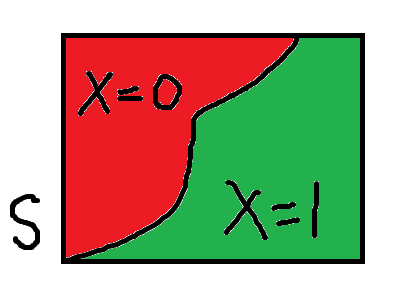
\includegraphics[width=80mm]{5.png}
\caption{Bernoulli Random Variable}
\end{figure}

Suppose the probability for ``success'' is $p$, PMF for $X$ is given by:

$$p_X(n)=P(X=n)=p^n(1-p)^{1-n}$$

where $p_X\in[0,1]$ and $n=0,1$, or alternatively:

$$p_X(1)=P(X=1)=p$$
$$p_X(0)=P(X=0)=1-p$$

The CDF $F_X(a)$ is given by

$$
F_X(a)=
\begin{cases} 
0 & a<0 \\
1-p & 0\le a<1 \\
1 & x \ge 1
\end{cases}
$$

\begin{figure}[H]
\centering
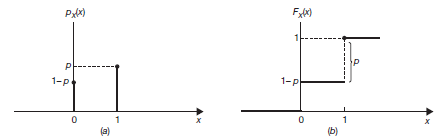
\includegraphics[width=120mm]{6.png}
\caption{Bernoulli Distribution}
\end{figure}

\subsubsection{Geometric Random Variable}

Suppose you are carrying out some number of Bernoulli trials that has a success rate of $q$ each time independently. You want to calculate the probability that after $n$ tries you achieved your first success. The probability is calculated as follows:

$$P(X=n)= \underbrace{ (1-q)(1-q) \cdots (1-q) }_{ \text{$n-1$ times} } q=(1-q)^{n-1} q$$

The suitable random variable for this problem is the geometric random variable $X \sim \text{Geom} (q)$. The possible values of $n$ are $1, 2, \dots$. Its PMF is given by

$$p_X(n)=P(X=n)=(1-q)^{n-1} q$$

where $p\in(0,1]$ and $n=1, 2,\dots$. Its CDF is given by

$$F_X(a)=1-(1-q)^a$$

where $a=1, 2,\dots$. \\

Note that this random variable is still discrete even though it can take infinitely many values because they take countably infinite integer values.

\begin{figure}[H]
\centering
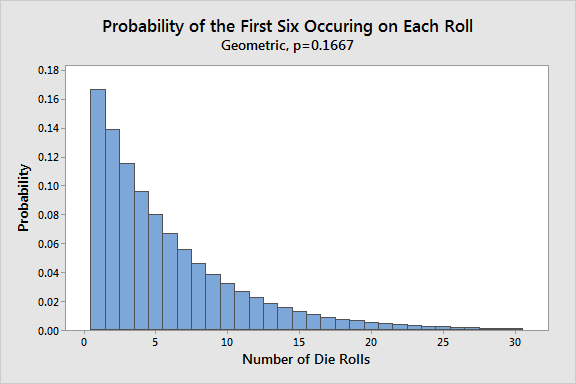
\includegraphics[width=120mm]{7.png}
\caption{Example Geometric PMF}
\end{figure}

\begin{figure}[H]
\centering
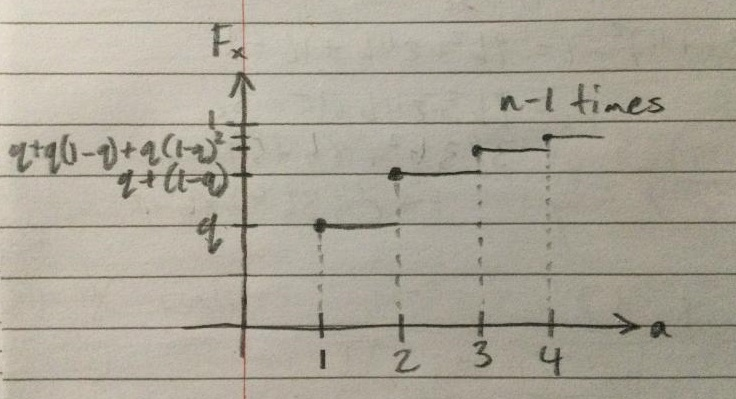
\includegraphics[width=120mm]{8.jpg}
\caption{Geometric CDF}
\end{figure}

For a discrete random variable, $\sum_i p_X (x_i)=1$ but for geometric random variable which is countably infinite,

$$\sum_{n=1}^\infty p_X(n) = \sum_{n=1}^\infty (1-q)^{n-1} q = 1$$

It can be proved using the formula for infinite geometric series:

\begin{align*}
\sum_{n=1}^\infty (1-q)^{n-1} q &= q \sum_{n=1}^\infty (1-q)^{n-1} \\
&= q \sum_{n=0}^\infty (1-q)^{n} \\
&= q\frac{1}{1-(1-q)} = 1
\end{align*}

A geometric random variable has something called \textit{memoryless property}. The idea is that if an experiment failed $n$ times then the probability that $m$ additional failures will happen is the same as the probability that the experiment failed $m$ times at the start. It indicates that the probability does not depend on past events. This property can be summarized by the below equation:

$$P(X>n+m\mid X>n)=P(X>m)$$

Explicit example: Consider an experiment of coin tosses and you happened to flip $5$ tails in a row and with that information, the probability of getting an additional $2$ tail is exactly the same as the probability of getting $2$ tails. \\

Also, note that

$$P(X>n+m\mid X>n)=P(X>n+m)$$

is not always true unless events $X>n+m$ and $X>n$ are independent (ie. $P(X>n)=1$). \\

\begin{figure}[H]
\centering
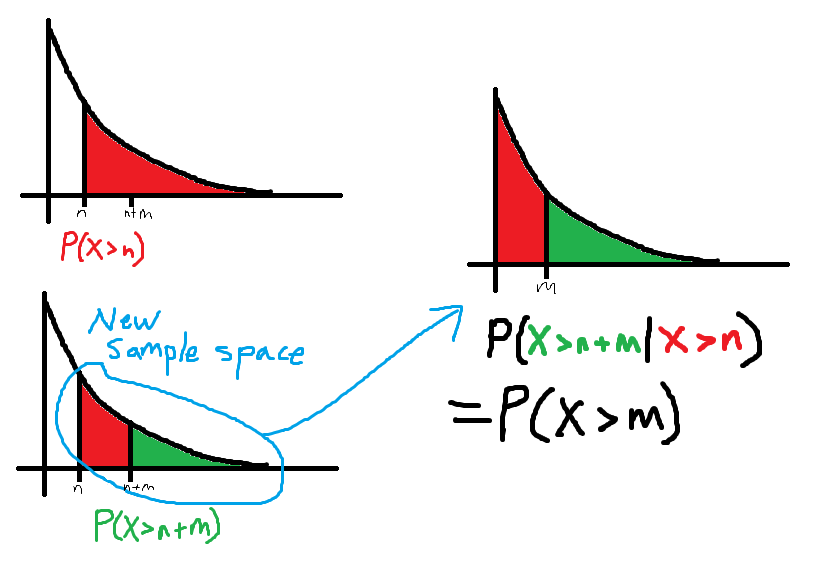
\includegraphics[width=120mm]{9.png}
\caption{Visualization for Memoryless Property on PDF}
\end{figure}

To prove the memoryless property, consider

\begin{align*}
P(X>n)&=\sum_{a=n+1}^\infty p_X(a)\\
&=\sum_{a=n+1}^\infty (1-q)^{a-1}q\\
&=q(1-q)^n\sum_{a = 0}^\infty (1-q)^a\\
&=(1-q)^n\sum_{a = 0}^\infty (1-q)^aq
\intertext{Since the sum of the whole PMF is one,}
&=(1-q)^n
\end{align*}

Applying the formula for conditional probability,

\begin{align*}
P(X>n+m\mid X>n)&=\frac{P(X>n+m\cap X>n)}{P(X>n)}\\
&=\frac{(1-q)^{n+m}}{(1-q)^n}\\
&=(1-q)^m=P(X>m)
\end{align*}

\subsubsection{Binomial Random Variable}

Binomial random variable $X\sim\text{Binom}(n,q)$ describes the number of successes if an experiment is repeated $n$ times, each with success rate $q$. Each experiment must be independent of each other. Examples of such experiments like coin flips or any experiment with binary outcomes. \\

Its PMF is given by

$$p_X(k)=P(X=k)={n \choose k} q^k(1-q)^{n-k}$$

where $k=0, 1, 2, \dots, n$. This formula gives the probability of getting exactly $k$ successes out of $n$ trials. \\

\begin{figure}[H]
\centering
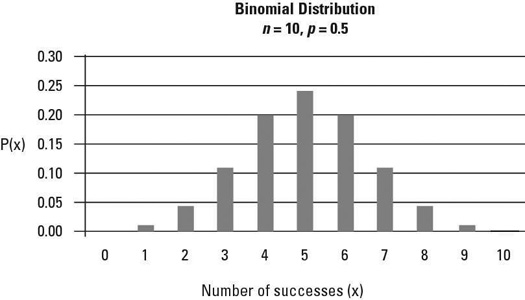
\includegraphics[width=120mm]{10.jpg}
\caption{Example binomial PMF}
\end{figure}

The below example will build intuition on where the formula came from.

\begin{texample}
Consider an unfair coin, let the probability of getting $H$ on a single toss be $0.6$ and the probability of getting $T$ is $0.4$. Find (1) the probability of obtaining the sequence $THHTTTHT$ (exactly, in this order) (2) the probability that a sequence of eight coin tosses would have $5$ tails and $3$ heads in any order. \\

(1) Coin toss events are independent of each other. The probability will be calculated as follows $0.4\cdot0.6\cdot0.6\cdot0.4\cdot0.4\cdot0.4\cdot0.6\cdot0.4=0.6^30.4^5=0.00221$. By symmetry, this is the same as the probability of getting the sequence $TTTTTHHH$ (or any other arrangements involving $3$ heads and $5$ tails) in exact order. \\

(2) The probability of getting $5$ tails and $3$ heads in any order can be calculated using the addition law for disjoint events:

\begin{align*}
P(\text{$3$ heads})&=P(\{THHTTTHT\}) + P(\{THTHTTTH\}) \\
&\quad+ P(\{TTHTHHTT\}) + \cdots \\
&\quad + P(\{\text{other arrangements of $3H$ and $5T$}\})
\end{align*}

In this case, we need to find the number of ways to permute $5$ tails and $3$ heads which is given by $\binom{8}{3}=56$. Using our answer to (1), the probability is therefore:

$$P(\text{$3$ heads})=56\cdot0.00221=0.12386$$
\end{texample}

The total probability of binomial PMF is indeed one:

$$\sum_{k=0}^{n} p_X(k) = \sum_{k=0}^{n} {n \choose k} q^k(1-q)^{n-k} = (q+(1-q))^n=1^n=1$$

\begin{texample}
Using the same unfair coin from the previous example, define a score to be (number of Heads) / (number of tosses). Find the probability that the score is between $0.4$ and $0.8$ when $N=9$ coins are tossed. What is the answer if $N$ is very large? \\

To get the score between $0.4$ and $0.8$, we need to get $4$ to $7$ heads. So the probability is

\begin{align*}
P(\text{score between 0.4 and 0.8})&=P(\text{4 or 5 or 6 or 7 heads}) \\
&= P(\text{4 heads})+P(\text{5 heads}) \\
&\quad + P(\text{6 heads})+P(\text{7 heads}) \\
&= \sum_{k=4}^7 \binom{9}{k}0.6^k0.4^{9-k} \\
&= 0.8301
\end{align*}

If $N$ is very large, the probability will reach $1$.
\end{texample}

\begin{texample}
You roll $5$ dice and what is the probability that you get $3$ sixes? \\

Let $X$ denote the number of sixes showing. There is $\frac16$ chance to roll six and $\frac56$ chance to roll other numbers. The probability of getting $3$ sixes is

$$P(X=3)={5\choose3}\left(\frac16\right)^3\left(\frac56\right)^2=0.032$$
\end{texample}

\subsubsection{Poisson Random Variable}

Poisson random variable $X\sim\text{Pois}(\lambda)$ can be used to find the probability of some number of events happening in some specified time period given that the event happens at some constant rate of $\lambda$ and the events occur independently. Its PMF is given by

$$p_X(n)=P(X=n)=e^{-\lambda}\frac{\lambda^n}{n!}$$

where $n=0,1,2,\dots$. It calculates the probability that $n$ events will happen at the specified time period. The parameter $\lambda>0$ can be thought as the mean number of event occurrences happening in the given time period. This PMF works because

$$\sum_{n=0}^\infty p_X(n) = \sum_{n=0}^\infty e^{-\lambda}\frac{\lambda^n}{n!} = e^{-\lambda} \sum_{k=0}^\infty \frac{\lambda^n}{n!}=e^{-\lambda}e^\lambda=1$$

The probability that $n$ events will happen in time interval $t$ given the event rate $r$ (the parameter is $\lambda=rt$) is

$$P(X=n)=e^{-rt}\frac{(rt)^n}{n!}$$

The possible examples of this random variable is not limited to the number of typos in a book, the number of radioactive decays in some time interval, and the number of people who failed exams. \\

Compared to binomial random variables which count discrete occurrences among discrete trials, the Poisson random variables count discrete occurrences among a continuous domain.

\begin{figure}[H]
\centering
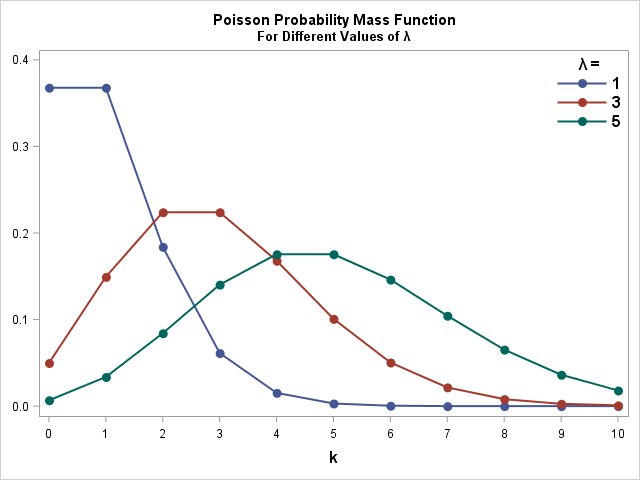
\includegraphics[width=100mm]{11.png}
\caption{Poisson PMFs for different values of $\lambda$. The PMF with $\lambda=3$ is peaked at $k=3$ which makes sense because events with the mean number of occurrences $\lambda=3$ per time frame of $10$ will most likely happen at $3$ times out of $10$.}
\end{figure}

When the number of trials $n$ of a binomial random variable approaches infinity and the probability of success $p$ approaches zero, it can be approximated with Poisson random variable with parameter $\lambda=pn$. This is a very robust approximation. \\

Consider a binomial random variable $X\sim\text{Binom}(n,q)$, applying $\lambda=pn$ to its distribution gives

\begin{align}
P(X = k) &= {n \choose k}p^k(1-p)^{n-k} \\
&=\frac{n(n-1)(n-2)\cdots(n-k+1)}{k!}\frac{\lambda^k}{n^k}\left(1-\frac{\lambda}{n}\right)^{n-k} \\
&=\frac{n(n-1)(n-2)\cdots(n-k+1)}{n^k}\frac{\lambda^k}{k!}\left(1-\frac{\lambda}{n}\right)^n\left(1-\frac{\lambda}{n}\right)^{-k}
\end{align}

Now as $n \to \infty$ and $p \to 0$, we have

$$\frac{n(n-1)(n-2)\cdots(n-k+1)}{n^k} \approx 1 \quad \left(1-\frac{\lambda}{n}\right)^n \approx e^{-\lambda} \quad \left(1-\frac{\lambda}{n}\right)^{-k} \approx 1$$

This gives

$$P(X = k) \approx \frac{\lambda^k}{k!}e^{-\lambda}$$

We get the Poisson approximation of $X$ as expected. We can see that Poisson random variables are great for modelling occurrences of events that could happen a very large number of times but happen rarely. Sometimes Poisson is preferred over binomial as they make calculations easier.

\begin{texample}
Birthday problem revisited: In a room of $n$ people, approximate the probability that at least $2$ people share the same birthday. \\

We will take a slightly different route from the last time. Imagine going over every possible pair of $n$ people and marking it off as a success when both of them share the same birthday. The probability of success happening is $\frac{1}{365}$. There are ${n \choose 2}$ possible pairs. \\

We can employ the Poisson approximation here. Let $X\sim\text{Pois}(\lambda)$ denote the number of pairs who share the same birthday where the average number of successful pairs is $\lambda={n \choose 2}\frac{1}{365}$. The probability that at least one pair share the same birthday is $P(X>0)=1-P(X=0)$ where $P(X=0)$ is the probability that none of the pairs share the same birthday. We get

$$P(X>0)=1-e^{-\lambda}=1-\exp\left( -{n \choose 2}\frac{1}{365} \right)$$

As an example, suppose $n=23$, $P(X>0)=0.5$. \\

The Poisson approximation can be generalized to more than two people. If we want to find the probability that at least three people share the same birthday, we only need modify the Poisson parameter which will be $\lambda={n \choose 3}\frac{1}{365^2}$ since we now need to choose three people and there is $\frac{1}{365^2}$ chance that three of them share the same birthday. \\

As a side note, binomial distribution cannot be used in this problem because it only works when events are independent which is not the case here. The probability of a person having a different birthday dependent on another person's birthday. But it is still ``possible'' to apply binomial distribution here since the Poisson's approximation works. For example if $n=23$, the probability is

$$P(X>0)=1-\left({n \choose 0} \left( p \right)^0 \left( 1-p \right)^{n}\right)=0.50048$$

where $n={23 \choose 2}$ and $p=\frac{1}{365}$. It is close enough to Poisson's approximation. This is only because $n$ is large and $p$ is small.
\end{texample}

\begin{texample}
You repeat an experiment $1000$ times, each with an independent success rate of $\frac{1}{500}$. Find the probability of getting at most two successes. \\

Denote $n=1000$ and $p=\frac{1}{500}$. One can use a binomial random variable to find probability:

\begin{align*}
P(\text{at most 2 success}) &= P(\text{0 success})+P(\text{1 success})+P(\text{2 success}) \\
&= \sum_{k=0}^2 {n\choose k} p^k (1-p)^{n-k} \\
&= 0.67668
\end{align*}

An even better way to solve is to approximate using a Poisson random variable $X\sim\text{Pois}(\lambda)$ where $\lambda=pn=2$. This gives

\begin{align*}
P(X \le 2)&=P(X=0)+P(X=1)+P(X=2) \\
&=e^{-\lambda}+e^{-\lambda}\frac{\lambda}{1}+e^{-\lambda}\frac{\lambda^2}{2}=5e^{-2} \\
&=0.67668
\end{align*}

This approximation works well because $n$ is large and $p$ is small.
\end{texample}

\subsubsection{Expectation Value}

The expectation value of a discrete random variable $X$ with corresponding PMF $p_X(x)$ is

$$E[X]=\sum_i x_i p_X(x_i)$$

It is the weighted average of all possible values $X$ can take $x_i$. It is denoted by either $E[X]$ (or simply $EX$) or $\langle X \rangle$. It is different from the average which is the mean result obtained after repeating an experiment for some number of times. But the average will become the expectation value if the experiment is repeated for infinite number of times (law of large numbers).

\begin{texample}
Let $X$ represent the outcome of a dice roll. Find its expectation value. \\

The possible values of $X$ are $x_i=1, 2, \dots, 6$ and the probability of rolling one of these values is $p_X(x_i)=\frac16$ so the expectation value is:

$$E[X]=\sum_{i=1}^6 x_i p_X(x_i)=1\frac16+2\frac16+3\frac16+4\frac16+5\frac16+6\frac16=3.5$$

It represents the average result you get if you roll the dice for infinite number of times.
\end{texample}

The expectation value for a Bernoulli random variable can be calculated in a straightforward manner as follows:

$$E[X\sim\text{Bern}(p)]=1p+0(1-p)=p$$

For geometric random variables, consider

$$f(x)=\sum_{n=0}^\infty x^n = \frac{1}{{1-x}} \quad f'(x)=\sum_{n=0}^\infty nx^{n-1} = \left(\frac{1}{{1-x}}\right)^2$$

Let $x=1-q$,

$$f'(1-q)=\sum_{n=0}^\infty n(1-q)^{n-1} = \frac{1}{q^2}$$

multiplying both sides by $q$ gives

$$q\sum_{n=0}^\infty n(1-q)^{n-1} = \sum_{n=0}^\infty nq(1-q)^{n-1} = \frac{1}{q}$$

This gives the closed formula for the expectation value of geometric random variables (remember that they start from $n=1$, not $n=0$):

$$E[X\sim\text{Geom}(q)]=\sum_{n=1}^\infty nq(1-q)^{n-1}=\frac1q$$

For binomial random variables, consider

$$\sum_{k=0}^n x^k p(k) = \sum_{k=0}^n {n \choose k} (qx)^k (1-q)^{n-k}=(1-q+qx)^n$$

taking a derivative with respect to x gives

$$\sum_{k=0}^n kx^{k-1} p(k) =n(1-q+qx)^{n-1}q$$

setting $x=1$,

$$\sum_{k=0}^n k p(k) =n(1)^{n-1}q=nq$$

This gives the expectation value for a binomial random variable

$$E[X\sim\text{Binom}(n,q)]=nq$$

Finally, for Poisson random variables, we start with

$$f(x)=\sum_n e^{-\lambda} \frac{\lambda^n}{n!}x^n$$

applying the Taylor expansion for $e^\lambda$,

$$f(x)=e^{-\lambda}e^{\lambda x}=e^{\lambda x-\lambda}$$

the derivative of $f(x)$ is

$$f'(x)=\lambda e^{\lambda x-\lambda}$$

Notice that $f(1)=1$, which is the total probability of Poisson PMF, and $f'(1)=\lambda$. This gives a Poisson random variable expectation

$$E[X\sim\text{Pois}(\lambda)]=\lambda$$

We see that the general strategy for finding closed-form expression for expectation is to start with a generating function of the following form

$$f(x)=\sum_n x^n p(n)$$

where $x$ takes values in $\mathbb{N}$. $f(1)=1$ represents the sum of probabilities. The derivative of this function is

$$f'(x)=\sum_n nx^{n-1} p(n)$$

$f'(1)$ usually gives the expectation value.

\subsection{Continuous Random Variables}

A random variable $X$ is said to be continuous if there exists a function $f_X(x)$ defined for all real numbers $x\in\mathbb{R}$ such that

$$P(X\in B)=\int_B f_X(x) dx$$

where $B$ is a set of real numbers.

\begin{figure}[H]
\centering
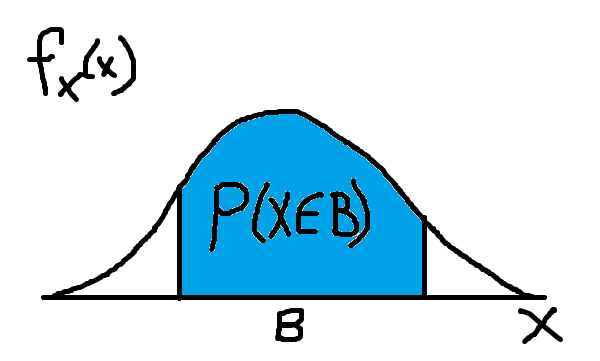
\includegraphics[width=100mm]{12.png}
\caption{Illustration of $P(X\in B)$}
\end{figure}

The function $f_X(x)$ is known as a probability density function PDF of $X$. It can be obtained as a derivative of CDF:

$$f_X(x)=\frac{d}{dx}F_X(x)$$

given that $F_X(x)$ is continuous and differentiable everywhere. The requirements for $f_X(x)$ include

\begin{enumerate}[i]
  \item $f_X(x) \ge 0$ for all $x$
  \item $f_X(x)$ must be (piecewise) continuous for all $x$
  \item $\displaystyle \int_{-\infty}^\infty f_X(x) dx = 1$
\end{enumerate}

$f_X(x)$ can have $f_X(x)>1$ for some $x$ values since it is not a probability function. The CDF of $X$ can be readily obtained by

$$F_X(a)=P(X\le a)=\int_{-\infty}^a f_X(x) dx$$

The probability of a continuous random variablele $X$ in range $(a,b)$ is

$$P(a < X < b)=P(a \le X < b)=P(a < X \le b)=P(a \le X \le b)=\int_a^b f_X(x) dx = F_X(b)-F_X(a)$$

It follows that the probability of $X$ takes any specific $a$ value is

$$P(X=a)=\int_{a}^a f_X(x) dx=0$$

Note that even though the probability is zero, it is still possible for $X$ to take $a$. This is because $X$ can take infinitely many values in range $(-\infty,\infty)$ which makes the size of sample space infinite. The probability of landing on a specific $a$ in this infinite sample space is very very low so the probability is zero but it does not make it impossible. \\

We will look over some special continuous random variables.

\subsubsection{Continuous Uniform Random Variable}

A continuous uniform distribution random variable $X\sim U(a, b)$ over the interval $[a,b]$ is described by the following PDF

$$
f_X(x)=\begin{cases}
\frac{1}{b - a} & a \le x \le b \\
0 & x<a\ \mathrm{or}\ x>b
\end{cases}
$$

\begin{figure}[H]
\centering
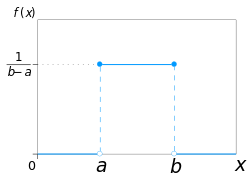
\includegraphics[width=100mm]{13.png}
\caption{PDF for Continuous Uniform Distribution}
\end{figure}

It can be used to model outcomes that lie in some boundary. The total probability is $1$ as expected because the area of the rectangular region is

$$(b-a)\frac{1}{b-a}=1$$

\subsubsection{Exponential Random Variable}

An exponential random variable $X\sim\text{Exp}(\lambda)$ of parameter $\lambda$ is described by the PDF

$$
f_X(x)=\begin{cases}
\lambda  e^{-\lambda x} & x \ge 0 \\
0 & x < 0
\end{cases}
$$

\begin{figure}[H]
\centering
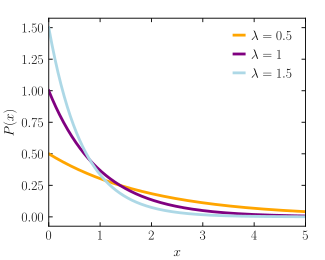
\includegraphics[width=100mm]{14.png}
\caption{PDF for Exponential Distribution}
\end{figure}

This distribution is often used to find waiting times for periodic events. As an example suppose in a certain country (Japan I think), there is an earthquake that happens every ten years. Define $\lambda$ (in fact it is the same one used in Poisson's) as the number of earthquakes happening every year which is $\lambda=\frac{1}{10}$. Let the random variable $X$ denote waiting time in years. The probability that the earthquake happens in less than five years is

$$P(X\le5)=\int_0^5\lambda e^{-\lambda x}dx=0.393$$

and the probability that you need to wait more than a year to see the earthquake happen is

$$P(X>1)=1-P(X\le1)=1-\int_0^1\lambda e^{-\lambda x}dx=0.9048$$

Note that you can calculate the same probability using a Poisson random variable with the same parameter. Redefine $X$ as the number of earthquakes happening in a one-year timespan. The probability that there are no earthquakes in one year is

$$P(X=0)=e^{-\lambda}=0.9048$$

It gives the same result! An exponential distribution's ``waiting time'' does not have any events happening, hence in the Poisson distribution we set the number of events happening in that time period to zero $X=0$. \\

The other applications of exponential distributions include finding the half-life of radioactive material. These problems can be modelled as finding time $a$ such that

$$P(X\ge a)=\frac12$$

$a$ can be found by

$$e^{-\lambda a}=\frac12$$

which gives $a=\frac{\ln(2)}{\lambda}$. \\

The total probability of the exponential distribution is indeed one:

$$\int_{-\infty}^\infty f_X(x) dx = \int_0^\infty \lambda e^{-\lambda x} dx = \left. -e^{-\lambda x} \right\vert_0^\infty = 1$$

Exponential distributions also have memoryless property like geometric random variables. The waiting time for a future event does not depend on elapsed time:

$$P(X\ge s+t \mid X\ge s)=P(X\ge t)$$

\begin{proof}
Evaluating $P(X\ge t)$ gives

$$P(X\ge t)=\int_t^\infty \lambda e^{-\lambda x} dx = \left. -e^{-\lambda x} \right\vert_t^\infty = e^{-\lambda t}$$

It also follows that

$$P(X\ge s)=e^{-\lambda s} \quad P(X\ge s+t)=e^{-\lambda (s+t)}$$

Using the definition of conditional probability to calculate $P(X\ge s+t \mid X\ge s)$ gives

$$P(X\ge s+t \mid X\ge s)=\frac{P(X\ge s+t)}{P(X\ge s)}=\frac{e^{-\lambda (s+t)}}{e^{-\lambda s}}=e^{-\lambda t}$$

this is the same as $P(X\ge t)$ which concludes the proof.
\end{proof}

As a supplement, we will show how Poisson distribution is used to derive exponential distribution. Let $X$ denote number of years. We saw earlier in the earthquake example that the probability that no earthquakes happen in one year is $e^{-\lambda}$. Now the probability that no earthquakes happen in $x$ years is just

$$P(X>x)=\underbrace{e^{-\lambda}e^{-\lambda}\cdots e^{-\lambda}}_{\text{$x$ times}}=e^{-\lambda x}$$

This allows us to define exponential distribution's CDF which is given by

$$F_X(x)=P(X\le x)=1-P(X>x)=1-e^{-\lambda x}$$

Finally we obtain exponential PDF by differentiating the CDF:

$$f_X(x)=\frac{d}{dx}F_X(x)=\lambda e^{-\lambda x}$$

\subsubsection{Normal Random Variable}

A normal random variable $X\sim N(\mu,\sigma^2)$ of mean $\mu$ and variance $\sigma^2$ is described by the following PDF:

$$f_X(x)=\frac{1}{\sigma\sqrt{2\pi}}\exp\left(-\frac12 \left( \frac{x-\mu}{\sigma} \right)^2\right)$$

It produces the famous bell curve

\begin{figure}[H]
\centering
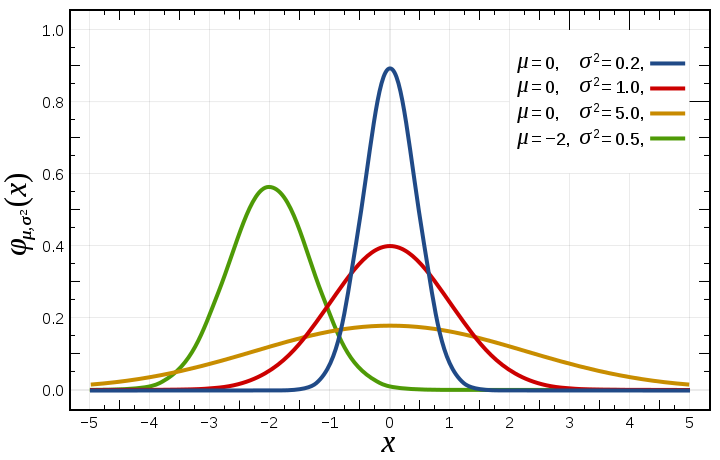
\includegraphics[width=100mm]{15.png}
\caption{Normal PDF. $\mu$ specifies the center of mass of the distribution and $\sigma^2$ controls how wide the curve is. Bigger the $\sigma^2$ is, more flatter the curve becomes.}
\end{figure}

\begin{figure}[H]
\centering
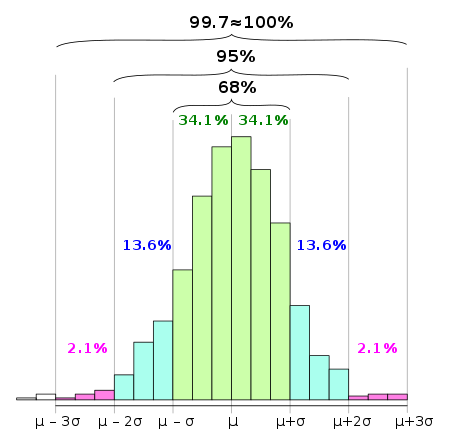
\includegraphics[width=120mm]{16.png}
\caption{Distribution of mass in Gaussian. One standard derivation $\sigma$ left and right from mean value $\mu$ will give about $68\%$ of the overall mass. Two standard derivations left and right from the mean will give about $95\%$ of the overall mass.}
\end{figure}

Like other distributions, the total probability of this distribution is indeed one.

\begin{proof}
\begin{align*}
\int_{-\infty}^\infty f_X(x) dx &= \frac{1}{\sigma\sqrt{2\pi}} \int_{-\infty}^\infty \exp\left(-\frac12 \left( \frac{x-\mu}{\sigma} \right)^2\right) dx
\intertext{Change of variables using $t=x-\mu$ gives}
&= \frac{1}{\sigma\sqrt{2\pi}} \int_{-\infty}^\infty \exp\left(-\frac{t^2}{2\sigma^2} \right) dt
\end{align*}

Denote the integral $\int_{-\infty}^\infty \exp\left(-\frac{t^2}{2\sigma^2} \right) dt$ by $I$. Integrating $I^2$ gives

\begin{align*}
I^2 &= \int_{-\infty}^\infty \exp\left(-\frac{x^2}{2\sigma^2} \right) dx \int_{-\infty}^\infty \exp\left(-\frac{y^2}{2\sigma^2} \right) dy \\
&= \int_{-\infty}^\infty \int_{-\infty}^\infty \exp\left(-\frac{x^2}{2\sigma^2} -\frac{y^2}{2\sigma^2} \right) dx dy
\intertext{We switch to polar coordinates}
&= \int_{0}^\infty \int_{0}^{2\pi} \exp\left(-\frac{r^2}{2\sigma^2} \right) r d\theta dr \\
&= 2\pi \int_{0}^\infty \exp\left(-\frac{r^2}{2\sigma^2} \right) rdr
\intertext{We make another change of variables using $u=\frac{r^2}{2\sigma^2}$ which gives}
&= 2\pi \int_0^\infty e^{-u} \sigma^2 du \\
&= 2\pi \sigma^2
\end{align*}

This gives $I=\sigma\sqrt{2\pi}$. Now

\begin{align*}
\int_{-\infty}^\infty f_X(x) dx = \frac{1}{\sigma\sqrt{2\pi}} I = \frac{1}{\sigma\sqrt{2\pi}} \sigma\sqrt{2\pi} = 1
\end{align*}
\end{proof}

The CDF for normal distribution is 

$$F_X(a)=P(X\le a)=\frac{1}{\sigma\sqrt{2\pi}} \int_{-\infty}^a \exp\left(-\frac12 \left( \frac{x-\mu}{\sigma} \right)^2\right) dx$$

There is no closed-form expression for $F_X(a)$. However, we can define standard normal $N(0, 1)$ whose PDF is

$$f_X(x)=\frac{\exp\left(-\frac{x^2}{2}\right)}{\sqrt{2\pi}}$$

and its CDF is

$$\phi(x) = \frac{1}{\sqrt{2\pi}}\int_{-\infty}^x \exp\left(-\frac{x^2}{2}\right) dx$$

Standard normal's CDF $\phi(x)$\footnote{In terms of error round function $\text{erf}$, $\phi$ can be written as $\phi(x)=\frac{1+\text{erf}(x/\sqrt{2})}{2}$.} can be used to calculate $F_X(a)$:

$$F_X(a)=\phi\left( \frac{a-\mu}{\sigma} \right)$$

\begin{figure}[H]
\centering
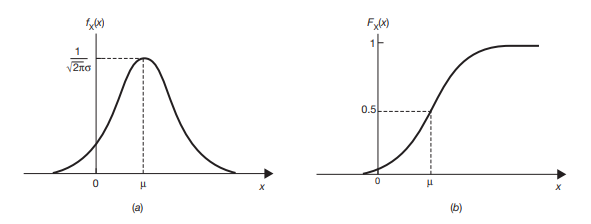
\includegraphics[width=120mm]{17.png}
\caption{Standard Normal's PDF and CDF}
\end{figure}

Normal random variable $X\sim N(\mu,\sigma^2)$ can be scaled to standard normal $Z\sim N(0,1)$ with $Z=\frac{X-\mu}{\sigma}$.

\begin{proof}
The probability of $Z\le t$ is

$$P(Z\le t)=\frac{1}{\sqrt{2\pi}}\int_{-\infty}^t \exp\left(-\frac{z^2}{2}\right) dz \quad\star$$

Since $X=\sigma Z+\mu$, $Z\le t$ is same as $X\le \sigma t+\mu$. So the probability of $X\le \sigma t+\mu$ is

$$P(X\le \sigma t+\mu)=\frac{1}{\sigma\sqrt{2\pi}} \int_{-\infty}^{\sigma t+\mu} \exp\left(-\frac12 \left( \frac{x-\mu}{\sigma} \right)^2\right) dx$$

Change of variables using $z=\frac{x-\mu}{\sigma}$\footnote{In statistics, $z$ is known as ``z-score.'' It measures how far $x$ deviates from mean $\mu$ in units of $\sigma$.} will convert this integral to the one marked with $\star$.
\end{proof}

Normal distributions have a broad range of applications everywhere. It is often used for random variables with unknown distribution patterns.

\begin{texample}
A group of programmers is trying to fix a buggy random number generator. They found that the mean of all generated random numbers is $310$ with standard deviation is $23$. What is the probability that it will generate a number somewhere between $250$ and $300$? \\

Let the normal random variable $X\sim N(310, 23^2)$ denote the random number generated. We want to calculate $P(250\le X\le 300)$. We can simplify the calculation using this substitution $Z=\frac{X-\mu}{\sigma}$ so the probability can be looked up using a standard normal table.

$$P(250\le X\le 300) = P(\frac{250-310}{23} \le \frac{X-\mu}{\sigma} \le \frac{300-310}{23}) = P(-2.61 \le Z \le -0.43)$$

Since the normal distribution is symmetric, $P(-2.61 \le Z \le -0.43)$ is same as $P(0.43 \le Z \le 2.61)$. The probability is

$$P(0.43 \le Z \le 2.61)=P(0 \le Z \le 2.61) - P(0 \le Z \le 0.43) \approx 0.4955 - 0.1664=0.3291$$
\end{texample}

\begin{texample}
A prisoner plays with a laser pointer in his jail cell. He randomly directs the laser beam at the wall one meter away from him.

\begin{figure}[H]
\centering
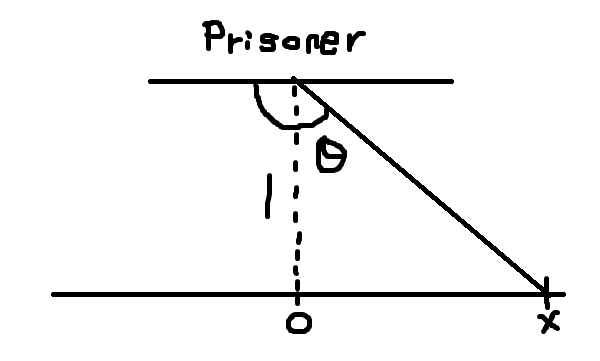
\includegraphics[width=80mm]{18.png}
\caption{Prisoner Playing with Laser}
\end{figure}

The laser beam angle $\theta$ is uniform in $[0, \pi]$. A security guard wants to find the most likely distance $x$ from origin $O$ where the laser beam lands. \\

Let random variable $X$ denote the distance from the origin. We need to find CDF for $X$:

$$F_X(x)=P(X\le x)$$

We can calculate $P(X\le x)$ using geometry. $x$ is some arbitrary distance from origin. From the diagram when the laser beam hits $x$, its angle is $\arctan x+\frac{\pi}{2}$. When $X\le x$, it follows that the angle $\theta \le \arctan x+\frac{\pi}{2}$. The probability that $X\le x$ is:

$$P(X\le x)=P(\theta \le \arctan x+\frac{\pi}{2})=\frac{1}{\pi}\left( \arctan x+\frac{\pi}{2} \right)=\frac{1}{\pi}\arctan x+\frac12$$

The PDF for $X$ can be obtained by differentiating $F_X(x)$:

$$f(x)=\frac{d}{dx}F_X(x)=\frac{1}{\pi (1+x^2)}$$

This is also the PDF for the standard Cauchy distribution.

\begin{figure}[H]
\centering
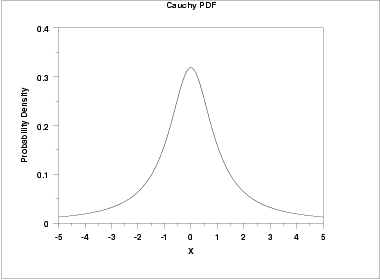
\includegraphics[width=100mm]{19.png}
\caption{Standard Cauchy PDF}
\end{figure}

The laser beam will most likely hit somewhere around $x=0$.
\end{texample}

\subsubsection{Expectation Value}

For continuous random variables $X$ with PDF $f(x)$, its expectation is defined as

$$E[X]=\int_{-\infty}^\infty xf(x) dx$$

Expectation for continuous uniform random variables can be calculated as follows:

$$E[X\sim U(a,b)]=\int_{-\infty}^\infty xf(x) dx=\int_a^b \frac{a}{b-a} dx=\frac{a+b}{2}$$

For exponential random variables, straightforward integration by parts gives

\begin{align*}
E[X\sim\text{Exp}(\lambda)]&=\int_0^\infty x\lambda e^{-\lambda x} dx \\
&=\left. -xe^{-\lambda x} \right\vert_0^\infty + \int_0^\infty e^{-\lambda x} dx \\
&=\frac{1}{\lambda}
\end{align*}

For normal random variables,

$$E[X\sim N(\mu, \sigma^2)]=\mu$$

I leave the calculation details for the readers. \\

\subsection{More on Expectation}

\begin{theorem}
If a continuous random variable $X \ge 0$, then

\[ EX=\int_0^\infty P(X\ge t) dt \]
\end{theorem}

\begin{proof}
\[ EX = \int_0^\infty P(X\ge t) dt = \int_0^\infty 1-F_X(t) dt \]

where $F_X(t)$ is CDF of $X$. Integrating by parts using $u=1-F_X(t)$ and $dv=dt$ gives

\[ EX = \left. t (1-F_X(t)) \right\vert_0^\infty + \int_0^\infty t f_X(t) dt \]

where $f_X(t)=\frac{d}{dt}F_X(t)$ is PDF for $X$. Provided that $\lim_{t\to\infty} t (1-F_X(t)) = 0$, we are left with

\[ EX = \int_0^\infty t f_X(t) dt \]
\end{proof}

If $X$ is a discrete random variable that takes values $0, 1, 2, \dots$,

\[ EX=\sum_{a=0}^\infty P(X>a) \]

\begin{theorem}
Law of the Unconscious Statistician: Let $g : \mathbb{R} \to \mathbb{R}$ be an only function and $X$ is a continuous random variable, then $g(X)$ is a new random variable. It follows that the expectation value for $g(X)$ is

\[ Eg(X)=\int_{-\infty}^\infty g(x) f(x) dx \]

If $X$ is discrete random variable,

\[ Eg(X)=\sum_i g(x_i) p(x_i) \]
\end{theorem}

\begin{proof}
If $g \ge 0$ then $g(X)\ge0$. The expectation for $g(X)$ is

\[ Eg(X)=\int_0^\infty P(g(x)\ge t) dt \]

Define a set $B_t=\{ x : g(x)\ge t \}$,

\[ Eg(X)=\int_0^\infty \int_{B_t} f(x) dx \: dt \]

\begin{figure}[H]
\centering
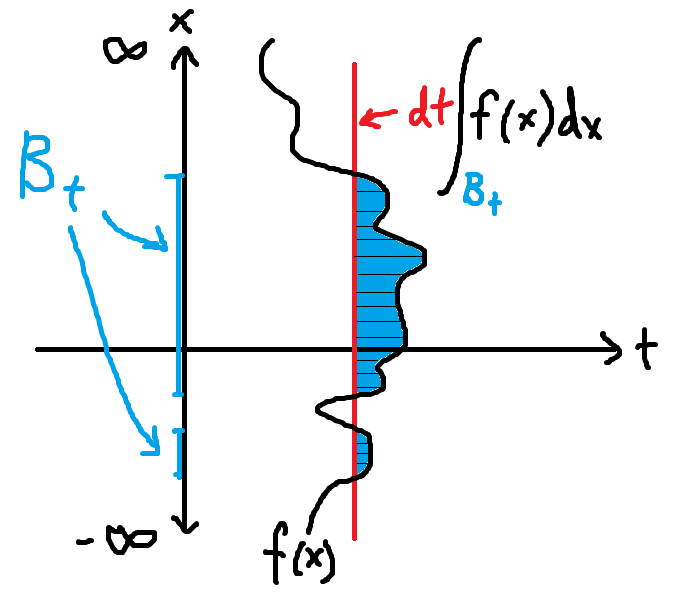
\includegraphics[width=100mm]{20.png}
\caption{Visualization of the integral $\displaystyle\int_0^\infty \int_{B_t} f(x) dx \: dt$}
\end{figure}

Changing the integration order gives

\[ Eg(X)=\int_{-\infty}^\infty \int_0^{g(x)} f(x) dt \: dx = \int_{-\infty}^\infty g(x) f(x) dx \]
\end{proof}

There is an important special case to consider: Let $a$ and $b$ denote constants. Suppose $g(X)=aX+b$,

\[ E(aX+b)=\int (ax+b)f(x)dx=a\int xf(x)dx+b\int f(x) dx = aEX+b \]

(The whole integral of the PDF is one: $\int_{-\infty}^\infty f(x) dx=1$.) This shows that expectation is linear.

\subsection{Moment and Variance}

The nth moment of a random variable $X$ is defined as

\[ E(X^n)=\begin{cases} \displaystyle\int_{-\infty}^\infty x^n f(x) dx & \text{$X$ continuous} \\[20pt] \displaystyle\sum_i x_i^n p(x_i) & \text{$X$ discrete} \end{cases} \]

Note that $E(X^n) = (EX)^n$ is not true all the time. From the definition, it follows that mean $EX$ is the first moment of $X$. $EX$ is usually denoted by $\mu$. \\

The variance (or second central moment) of $X$ is defined as

\[ \text{Var}(X)=\sigma^2=E((x-\mu)^2) \]

$\text{Var}(X)$ is always greater than or equal to zero. The standard deviation is just the square root of variance: $\sigma=\sqrt{\text{Var}(X)}$. They both measure the spread of distribution from the mean. \\

Note that the following is equivalent

\[ \text{Var}(X)=E(X^2)-(EX)^2 \]

\begin{proof}
\begin{align*}
\text{Var}(X)&=E((x-\mu)^2) \\
&=E(x^2-2x\mu+\mu^2) \\
&=\int (x^2-2x\mu+\mu^2) f(x) dx \\
&=\int x^2 f(x) dx -2\mu\int xf(x) dx + \mu^2 \int f(x) dx \\
&=E(X^2)-2\mu EX + \mu^2 \\
&=E(X^2)-2(EX)^2+(EX)^2 \\
&=E(X^2)-(EX)^2
\end{align*}
\end{proof}

Variances for some random variables are given in the below table

\begin{center}
\begin{tabular}{| c | c |}
\hline
Random variable $X$ & $\text{Var}(X)$ \\
\hline
$\text{Binom}(n,p)$ & $np(1-p)$ \\
\hline
$\text{Pois}(\lambda)$ & $\lambda$ \\
\hline
$\text{Exp}(\lambda)$ & $\frac{1}{\lambda^2}$ \\
\hline
$N(\mu,\sigma^2)$ & $\sigma^2$ \\
\hline
\end{tabular}
\end{center}

\begin{theorem}
Let $a$ and $b$ denote constants,

\[ \text{Var}(aX+b)=a^2\text{Var}(X) \]

or variance is independent of $b$ added to $X$ (ie. invariant of location) and if $X$ is scaled by $a$, variance is scaled by $a^2$.
\end{theorem}

\begin{proof}
First, we prove that $\text{Var}(X+b)=\text{Var}(X)$,

\begin{align*}
\text{Var}(X+b)&=E((X+b)^2)-(E(X+b))^2
\intertext{Since expectation is linear operator: $E(X+b)=EX+b$,}
&=E(X^2+2bX+b^2)-(EX+b)^2 \\
&=E(X^2)+2b(EX)+b^2-((EX)^2+2b(EX)+b^2) \\
&=E(X^2)+2b(EX)+b^2-(EX)^2-2b(EX)-b^2 \\
&=E(X^2)-(EX)^2 \\
&=\text{Var}(X)
\end{align*}

Next, we prove that $\text{Var}(aX)=a^2\text{Var}(X)$,

\begin{align*}
\text{Var}(aX)&=E((aX)^2)-(E(aX))^2 \\
&=a^2E(X^2)-a^2(EX)^2 \\
&=a^2(E(X^2)-(EX)^2) \\
&=\text{Var}(X)
\end{align*}
\end{proof}

\subsection{Joint Distributions}

\subsubsection{Discrete Case}

Let $X,Y$ be discrete random variables, the function

\[ p_{XY}(x,y)=P(X=x,Y=y) \]

is called the joint PMF of $X$ and $Y$. \\

Joint PMFs share many properties with ordinary PMFs. For example, the total probability is one:

\[ \sum_i \sum_j p_{XY}(x_i,y_i) = 1 \]

To calculate the probability that $X$ takes values in range $[x_1, x_2]$ and $Y$ takes values in range $[y_1, y_2]$:

\[ P((x_1\le X\le x_2) \cap (y_1\le Y\le y_2)) = \sum_{x=x_1}^{x_2} \sum_{y=y_1}^{y_2} p_{XY}(x,y) \]

We can obtain PMF for $X$ alone from the joint PMF. It is called the marginal PMF of $X$ and is defined as

\[\ p_X(x)=P(X=x)=\sum_j p_{XY}(x,y_j) \]

Similarly for $Y$,

\[\ p_Y(y)=P(Y=y)=\sum_i p_{XY}(x_i,y) \]

The below shows an example joint PMF:

\begin{center}
    \begin{tabular}{|c|c|c|c|c|}
      \hline
      \diagbox{$Y$}{$X$} & $1$ & $2$ & $3$ & \\
      \hline
      $1$ & $1/4$ & $1/8$ & $1/8$ & $1/2$ \\
      \hline
      $4$ & $1/6$ & $1/3$ & $0$ & $1/2$ \\
      \hline
      & $10/24$ & $11/24$ & $3/24$ & \diagbox{$p_X$}{$p_Y$} \\
      \hline
    \end{tabular}
\end{center}

All of its entries sum up to one:

\[\frac14+\frac18+\frac18+\frac16+\frac13+0=1\]

Also, notice the total for $p_X$ and $p_Y$ add up to one as well.

\begin{texample}
You toss $4$ dice. Let random variables $X$ denote the number of distinct results and $Y$ denote the minimal result. Find $P(X=1,Y=3)$ and $P(X=4,Y=3)$. \\

$$P(1,3)=P(\{3, 3, 3, 3, 3\})=\frac{1}{6^4}$$

$$P(4, 3)=P(\text{roll $3,4,5,6$ in some order})=\frac{4!}{6^4}$$
\end{texample}

\subsubsection{Continuous Case}

Let $X,Y$ be continuous random variables, the function $f_{XY}(x,y)$ is called the joint PDF of $X$ and $Y$. The probability can be calculated as follows

\[ P((X,Y)\in A) = \iint_A f_{XY}(x,y) dx \:dy \]

\begin{figure}[H]
\centering
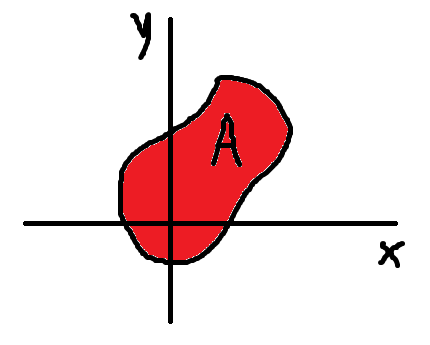
\includegraphics[width=100mm]{21.png}
\caption{Illustration of $A$}
\end{figure}

Joint PDFs share many properties with ordinary PDFs. For example, $f_{XY}(x,y)\ge0$ everywhere and

\[ \int_{-\infty}^\infty \int_{-\infty}^\infty f_{XY}(x,y) dx \:dy = 1 \]

To find the probability that $X$ takes values in range $[x_1, x_2]$ and $Y$ takes values in range $[y_1, y_2]$:

\[ P((x_1\le X\le x_2) \cap (y_1\le Y\le y_2)) = \int_{y_1}^{y_2} \int_{x_1}^{x_2} f_{XY}(x,y) dx \:dy \]

Marginal PDF for $X$:

\[ f_X(x)=\int_{-\infty}^\infty f(x,y) dy \]

Marginal PDF for $Y$:

\[ f_Y(y)=\int_{-\infty}^\infty f(x,y) dx \]

\begin{texample}
Consider the following joint PDF:

\[ f_{XY}(x,y)=\begin{cases} x+y & 0\le x,y \le1 \\ 0 & \text{otherwise} \end{cases} \]

\begin{center}
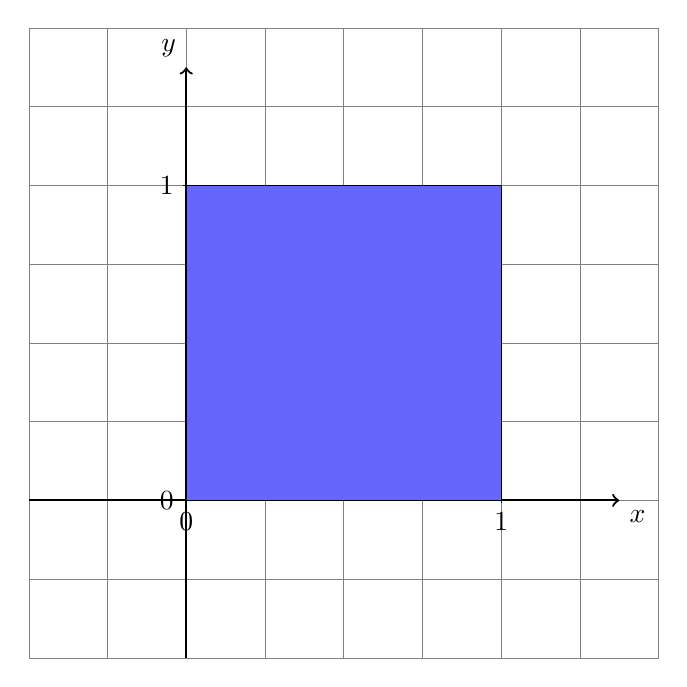
\begin{tikzpicture}
\draw[step=1cm,gray,very thin] (-2,-2) grid (6,6);
\draw[thick,->] (-2,0) -- (5.5,0) node[anchor=north west] {$x$};
\draw[thick,->] (0,-2) -- (0,5.5) node[anchor=south east] {$y$};
\foreach \x [count=\i from 0] in {0,4}
   \draw (\x cm,1pt) -- (\x cm,-1pt) node[anchor=north] {$\i$};
\foreach \y [count=\i from 0] in {0,4}
    \draw (1pt,\y cm) -- (-1pt,\y cm) node[anchor=east] {$\i$};
\filldraw[fill=blue!60!white, draw=black] (0,0) rectangle (4,4);
\end{tikzpicture}
\end{center}

Find the marginal PDF for $X$. \\

\[ f_X(x)=\int_{-\infty}^\infty f_{XY}(x,y) dy = \int_0^1 x+y\:dy = x+\frac12 \]

\begin{center}
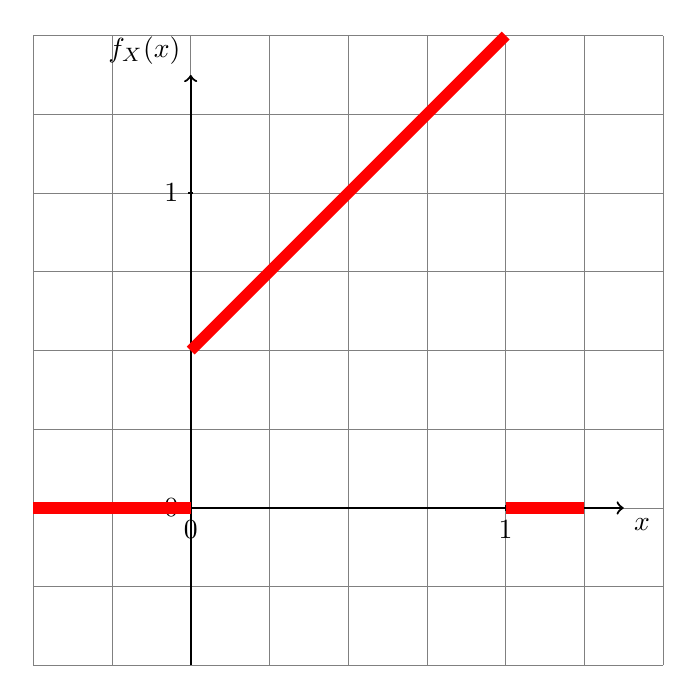
\begin{tikzpicture}
\draw[step=1cm,gray,very thin] (-2,-2) grid (6,6);
\draw[thick,->] (-2,0) -- (5.5,0) node[anchor=north west] {$x$};
\draw[thick,->] (0,-2) -- (0,5.5) node[anchor=south east] {$f_X(x)$};
\foreach \x [count=\i from 0] in {0,4}
   \draw (\x cm,1pt) -- (\x cm,-1pt) node[anchor=north] {$\i$};
\foreach \y [count=\i from 0] in {0,4}
    \draw (1pt,\y cm) -- (-1pt,\y cm) node[anchor=east] {$\i$};
\draw[line width=4pt,red] (-2,0) -- (0,0);
\draw[line width=4pt,red] (4,0) -- (5,0);
\draw[line width=4pt,red] (0,2) -- (4,6);
\end{tikzpicture}
\end{center}
\end{texample}

\subsubsection{Expectation}

If $X$ and $Y$ are random variables and $g$ is a function that takes these random variables, the expectation of $g(X,Y)$ is

\[ Eg(X,Y)=\sum_i \sum_j g(x_i,y_i)p(x_i,y_i) \]

for discrete random variables or

\[ Eg(x,y)=\int_{-\infty}^\infty \int_{-\infty}^\infty g(x,y)f(x,y) dx\:dy \]

for continuous random variables. For example, if $g(X,Y)=X+Y$, when $X$ and $Y$ are continuous,

\begin{align*}
E[X+Y]&=\int_{-\infty}^\infty \int_{-\infty}^\infty (x+y)f(x,y) dx\:dy\\
&=\int_{-\infty}^\infty \int_{-\infty}^\infty xf(x,y) dx\:dy+\int_{-\infty}^\infty \int_{-\infty}^\infty yf(x,y) dx\:dy\\
&=EX+EY
\end{align*}

It turns out that the linearity of expectation still holds for multiple random variables:

\[E\left(\sum_i a_i X_i \right) = \sum_i a_i E(X_i)\]

\subsubsection{Independence}

The random variables $X$ and $Y$ are independent if for any $a,b \in \mathbb{R}$,

\[ P(X\le a, Y\le b)=P(X\le a) P(Y\le b) \]

ie. events $X\le a$ and $Y\le b$ are independent. In terms of PMF and PDF, $X$ and $Y$ are independent if

\[p_{XY}(x,y)=p_X(x)p_Y(y)\]

for discrete case and

\[f_{XY}(x,y)=f_X(x)f_Y(y)\]

for continuous case. \\

For any functions $g(X)$ and $h(Y)$, there exists a simple formula for calculating $E[g(X)h(Y)]$ when $X$ and $Y$ are independent.

\begin{align*}
E[g(X)h(Y)]&=\int_{-\infty}^\infty \int_{-\infty}^\infty g(x)h(y) f(x,y) dx\: dy
\intertext{Since $X$ and $Y$ are independent, $f(x,y)=f_X(x)f_Y(y)$,}
&=\int_{-\infty}^\infty \int_{-\infty}^\infty g(x)h(y) f_X(x)f_Y(y) dx\: dy \\
&=\left( \int_{-\infty}^\infty g(x) f_X(x) dx \right) \left( \int_{-\infty}^\infty h(y) f_Y(y) dy \right) \\
&=E[g(X)]E[h(Y)]
\end{align*}

In particular, $E[XY]=E[X]E[Y]$. This works for discrete random variables as well.

\begin{texample}
Consider the following joint PMF

\[ p_{XY}(x,y)=\frac{x^2y}{30} \]

for discrete random variables $X=1,2$ and $Y=1,2,3$. Show that $X$ and $Y$ are independent. \\

The marginal PMF for $X$ is

\[p_X(x)=\sum_{y=1}^3 \frac{x^2y}{30} = \frac{x^2}{5}\]

The marginal PMF for $Y$ is

\[p_Y(y)=\sum_{x=1}^2 \frac{x^2y}{30} = \frac{y}{6}\]

Since

\[p_{XY}(x,y)=p_X(x)p_Y(y)=\frac{x^2y}{30}\]

So $X$ and $Y$ are independent.
\end{texample}

\subsubsection{Covariance and Correlation Coefficient}

Covariance between two random variables $X$ and $Y$ is defined as

\[ \text{Cov}(X,Y)=E[(X-EX)(Y-EY)] \]

In particular, $\text{Cov}(X,X)=\text{Var}(X)$. There is another formula for covariance:

\begin{align*}
\text{Cov}(X,Y)&=E[(X-EX)(Y-EY)] \\
&=E[XY-(EX)Y-X(EY)+(EX)(EY)] \\
&=E[XY]-E[X]E[Y]-E[X]E[Y]+E[X]E[Y] \\
&=E[XY]-E[X]E[Y]
\end{align*}

\footnote{$\displaystyle E[XY]=\sum_i \sum_j x_iy_ip_{XY}(x_i,y_j)$} It follows that if $X$ and $Y$ are independent, $\text{Cov}(X,Y)=0$ since $E[XY]=E[X]E[Y]$.

\begin{texample}
Consider discrete random variables $X$ and $Y$, Their joint PMF is specified below

\begin{center}
    \begin{tabular}{|c|c|c|}
      \hline
      \diagbox{$Y$}{$X$} & $0$ & $1$ \\
      \hline
      $-1$ & $0$ & $1/4$ \\
      \hline
      $1$ & $1/2$ & $1/4$ \\
      \hline
    \end{tabular}
\end{center}

Find $\text{Cov}(X,Y)$. \\

We have
\[EX=0 \cdot \frac12 + 1 \cdot \left(\frac14+\frac14\right)=\frac12\]

\[EY=-1\cdot \frac14+1\cdot\left(\frac12+\frac14\right)=\frac12\]

\[E[XY]=-1\cdot\frac14+1\cdot\frac14=0\]

Covariance of $X$ and $Y$ is therefore

\[\text{Cov}(X,Y)=E[XY]-EXEY=0-\frac12\cdot\frac12=-\frac14\]

\end{texample}

Covariance measures how much two random variables are \textit{linearly} related to each other (correlation). Positive covariance indicates that one variable is related to another variable linearly (e.g. when one variable is large, the other variable will also be large). The bigger the covariance is, the stronger the linear relationship becomes. Negative covariance indicates that there is an inverse linear relationship between two variables (eg. when one variable is small another variable will be big, and vice versa). When covariance is zero, $X$ and $Y$ do not have some linear relationship (ie. uncorrelated), but it does not necessarily imply that $X$ and $Y$ are independent. Again, consider continuous random variables $X \sim U(-1,1)$ and $Y=X^2$. They are clearly dependent since $Y$ depends on the value of $X$\footnote{Note that you can't conclude that they are independent just because $E[XY]=E[X]E[Y]$. If $X$ and $Y$ are independent then $E[XY]=E[X]E[Y]$ but it is not necessarily true that if $E[XY]=E[X]E[Y]$ then $X$ and $Y$ are independent, only imply uncorrelateness.}.

\begin{texample}
Show that $X$ and $Y$ are not independent. \\

Independence means $P(X\le a, Y\le b)=P(X\le a) P(Y\le b)$ for any real numbers $a$ and $b$. Consider $a=\frac13$ and $b=\frac 14$. \\

- $X \le \frac 13$, i.e. when $-1 \le X \le \frac13$, has probability $\frac{1+\frac13}{2}=\frac23$ \\
- $Y \le \frac 14$, i.e. when $-\frac12 \le X \le \frac12$, has probability $\frac12$ \\
- $X \le \frac 13, Y \le \frac 14$ together, i.e. when $-\frac12 \le X \le \frac13$, has probability $\frac5{12}$ \\

but $\frac23 \times \frac12 \not=\frac5{12}$. This makes $X$ and $Y$ not independent.
\end{texample}

So, we have

$$E[X] = 0$$
$$E[Y] = E[X^2] = \int_{-1}^{1} x^2  dx = \frac23$$
$$E[XY] = E[X^3] = \int_{-1}^{1} x^3 dx = 0$$

The covariance is therefore

\[ \text{Cov}(X,Y) = E[X^3] - E[X] E[X^2] = 0 - 0 \cdot \frac23 = 0 \]

This means $X$ and $Y$ do not depend on each other linearly.

\begin{figure}[H]
\centering
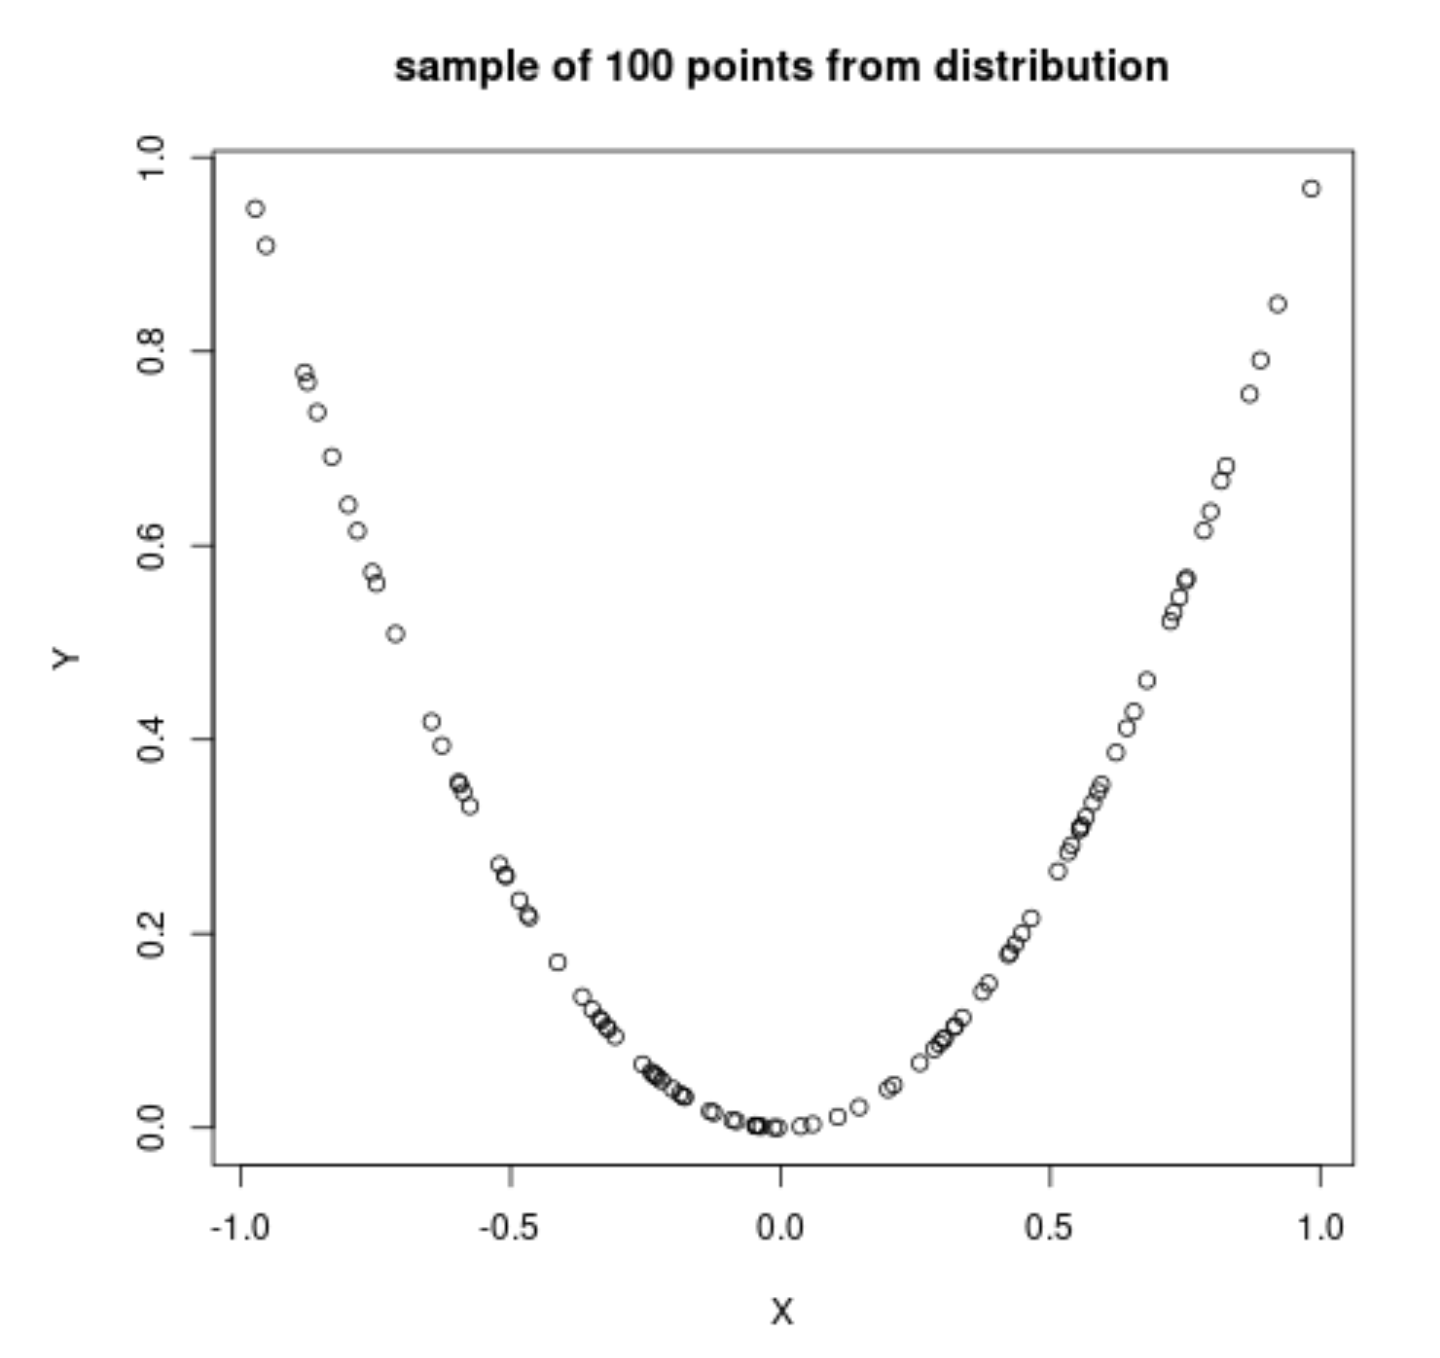
\includegraphics[width=100mm]{22.png}
\caption{Sample of $1000$ points from the distribution. Points depend on each other quadratically but not linearly.}
\end{figure}

\begin{texample}
Suppose $5$ cards are drawn from the standard deck of $52$ cards. Denote random variables $X$ to be the number of spades in the hand and $Y$ to be the number of black cards in the hand. Calculate $\text{Cov}(X,Y)$. \\

Let's try calculating $P(X=2,Y=4)$, the probability that a poker hand contains $4$ black cards and $2$ spades first. There are ${52 \choose 5}$ ways to choose $5$ cards from the deck, ${13\choose2}$ ways to select 2 spades, ${13\choose2}$ ways to select the remaining 2 black cards excluding spades, and ${26\choose1}$ ways to choose a red card. The probability is

\[ P(X=2,Y=4)=\frac{{13\choose2}{13\choose2}{26\choose1}}{{52\choose5}} \]

We can generalize this result to $x$ spades and $y$ black cards to create the joint PMF for $X$ and $Y$:

\[ p_{XY}(x,y)=P(X=x,Y=y)=\frac{{13\choose x}{13\choose y-x}{26\choose 5-y}}{{52\choose5}} \]

This gives nonzero probability when $X\le Y$. The joint PMF table is given below:

\begin{center}
\footnotesize
\begin{tabular}{|c|c|c|c|c|c|c|c|}
\hline
\diagbox{$Y$}{$X$} &         $0$&         $1$&         $2$&         $3$&         $4$&         $5$& \\
\hline
$0$ & $0.025310$ & $0.000000$ & $0.000000$ & $0.000000$ & $0.000000$ & $0.000000$ & $0.02531$ \\
\hline
$1$ & $0.074780$ & $0.074780$ & $0.000000$ & $0.000000$ & $0.000000$ & $0.000000$ & $0.14956$ \\
\hline
$2$ & $0.078031$ & $0.169068$ & $0.078031$ & $0.000000$ & $0.000000$ & $0.000000$ & $0.32513$ \\
\hline
$3$ & $0.035764$ & $0.126801$ & $0.126801$ & $0.035764$ & $0.000000$ & $0.000000$ & $0.32513$ \\
\hline
$4$ & $0.007153$ & $0.037195$ & $0.060864$ & $0.037195$ & $0.007153$ & $0.000000$ & $0.14956$ \\
\hline
$5$ & $0.000495$ & $0.003576$ & $0.008583$ & $0.008583$ & $0.003576$ & $0.000495$ & $0.02531$ \\
\hline
& $0.221534$ & $0.411420$ & $0.274280$ & $0.081543$ & $0.010729$ & $0.000495$ & \diagbox{$p_X$}{$p_Y$} \\
\hline
\end{tabular}
\end{center}

With expectation values

\[EX=1.25\]
\[EY=2.5\]

There are two ways to calculate covariance: use $E[(X-EX)(Y-EY)]$ or $E[XY]-E[X]E[Y]$. Both methods give the same answer:

\[\text{Cov}(X,Y)=\sum_{y=0}^5\sum_{x=0}^5 (x-EX)(y-EY) p_{XY}(x,y)=0.575980\]

\[\text{Cov}(X,Y)=\left( \sum_{y=0}^5\sum_{x=0}^5 xyp_{XY}(x,y) \right)-(EX)(EY)=0.575980\]

When the number of spades increases, the number of black cards also increases. \\

Most of the computations in this example are handled by Python\footnote{\href{https://gist.github.com/marethyu/777e372c69cb356c5fc8c93f59cf62e6}{Source code}}.
\end{texample}

Correlation coefficient $\rho(X,Y)$ of $X$ and $Y$ is defined as

\[\rho(X,Y)=\frac{\text{Cov}(X,Y)}{\sqrt{\text{Var}(X)\text{Var}(Y)}}\]

It is a unitless quantity that measures correlation between $X$ and $Y$. It can be thought as the a normalized version of covariance since it takes values between $-1$ and $1$. To prove this statement, consider the following theorem:

\begin{theorem}
Cauchy-Schwarz Inequality: $|E(XY)|^2 \le E(X^2)E(Y^2)$
\end{theorem}

\begin{proof}
Define a new random variable $Z=X+\lambda Y$ where $\lambda$ is some real number. \\

The expectation for $Z^2$ is

\begin{align*}
E(Z^2)&=E((X+\lambda Y)^2) \\
&=E(X^2+2\lambda XY+\lambda^2Y^2) \\
&=E(X^2)+2\lambda E(XY)+\lambda^2 E(Y^2)
\end{align*}

Clearly, $E(Z^2)$ cannot be less than 0: $E(Z^2)\ge0$. Let $c=E(X^2)$, $b=2E(XY)$ and $a=E(Y^2)$,

\[ a\lambda^2+b\lambda+c\ge0 \]

Recall that a quadratic equation that gives positive values for all $\lambda$ should have discriminant $b^2-4ac \le 0$. This means

\[(2E(XY))^2-4E(X^2)E(Y^2)\le0\]
\[E(XY)^2-E(X^2)E(Y^2)\le0\]

We finally get the equality:

\[|E(XY)|^2 \le E(X^2)E(Y^2)\]

\end{proof}

We will now apply this inequality to show that $\rho(X,Y)$ is normalized.

\begin{theorem}
$\rho(X,Y)$ only takes values between $-1$ and $1$.
\end{theorem}

\begin{proof}
We know that $\text{Cov}(X,Y)=E[(X-EX)(Y-EY)]$. Applying the Cauchy-Schwarz inequality to $E[(X-EX)(Y-EX)]$ gives

\[|E[(X-EX)(Y-EY)]|^2 \le E[(X-EX)^2]E[(Y-EY)^2]\]

By the definition of variance,

\[|\text{Cov}(X,Y)|^2 \le \text{Var}(X)\text{Var}(Y)\]

\[\frac{|\text{Cov}(X,Y)|^2}{\text{Var}(X)\text{Var}(Y)} \le 1\]

Taking square root gives

\[|\rho| \le 1\]

So $-1\le\rho\le1$.
\end{proof}

It can be shown that

\[\rho(X,Y)=\begin{cases} 1 & \text{iff $Y=aX+b$ where $a,b\in\mathbb{R}$ and $a>0$} \\[20pt] -1 & \text{iff $Y=aX+b$ where $a,b\in\mathbb{R}$ and $a<0$} \end{cases}\]

In other words, $|\rho|=1$ if there is a direct linear relationship between $X$ and $Y$.

\subsubsection{Variance and Independence}

\begin{theorem}
If $X,Y$ are independent then

\[\text{Var}(X+Y)=\text{Var}(X)+\text{Var}(Y)\]
\end{theorem}

\begin{proof}
\begin{align*}
\text{Var}(X+Y)&=E((X+Y)^2)-(E(X+Y))^2 \\
&=E(X^2+2XY+Y^2)-(EX+EY)^2 \\
&=E(X^2)+2E(XY)+E(Y^2)-((EX)^2+2(EX)(EY)+(EY)^2) \\
&=(E(X^2)-(EX)^2)+(E(Y^2)-(EY)^2)+2(E(XY)-(EX)(EY)) \\
&=\text{Var}(X)+\text{Var}(Y)+2\text{Cov}(X,Y)
\intertext{Since $X,Y$ are independent, $\text{Cov}(X,Y)=0$,}
&=\text{Var}(X)+\text{Var}(Y)
\end{align*}
\end{proof}

This result can be generalized to multiple random variables:

\[\text{Var}\left( \sum_i X_i \right) = \sum_i \text{Var}(X_i)\]

\begin{texample}
Find variance for a binomial random variable $X\sim\text{Binom}(n,p)$. \\

We can write $X$ in terms of $n$ independent Bernoulli trials:

\[X=X_1+X_2+\cdots+X_n\]

where $X_i$ are Bernoulli random variables. \\

Since $X_i$s are independent from each other,

\[\text{Var}(X)=\text{Var}\left( \sum_{i=1}^n X_i \right) = \sum_{i=1}^n \text{Var}(X_i)\]

For a single trial, the variance is

\[\text{Var}(X_i)=E(X_i^2)-(E(X_i))^2\]

Since $X_i^2=X_i$ and expectation for Bernoulli random variable is $p$,

\[\text{Var}(X_i)=E(X_i)-(E(X_i))^2=p-p^2\]

The variance for a binomial random variable is therefore

\[\text{Var}(X) = \sum_{i=1}^n p-p^2 = np(1-p)\]
\end{texample}

\end{document}